
%==============================================================================
%
%      File:  Master.TEX  (Stored in TEX$LATEX: as UNHTHESIS.TEMPLATE)
%  Language:  LaTeX - Document Preparation System
%      Date:  26/Dec/2005
%    Author:  Maha El Meseery
%             
%
%   This document  is my master thesis on sketch Recognition and understanding
%
%
%        % latex mythesis
%
%------------------------------------------------------------------------------

%    14 Aug 02 Updated document to latex 2e. Also, changed wording 
%              to be consistent with an X windows system.

%    14 Aug 02 Added \includeonly command in comments.



% During the editing process you will not want to view and print the
% whole document. Uncomment the command below so that only the
% chapters that you want to work on are visible.
%\includeonly{ChapterIntroduction}
%\documentstyle[11pt,unhthesis]{report}
\documentclass[11pt,doublespace]{SketchThesis}


% Extra modules can be added to your document to extend the things
% the Latex can Do. One of these is psfig which allows you to print
% postscript files. You tell Latex to read these packages using the
% \usepackage command:
%\usepackage{setspace}
\usepackage{psfig}
\usepackage{named}
\usepackage{natbib}
\bibliographystyle{plain}
\hyphenation{gno-mon-ly}
%\usepackage{setspace}
\usepackage {graphicx}
\usepackage{subfigure}
\usepackage{longtable}
\usepackage{lscape}
\usepackage{array}
\usepackage{algorithmic}
\usepackage{algorithm} 
%\numberwithin{algorithm}{chapter}
%\usepackage[T1]{fontenc}
\usepackage[latin9]{inputenc}


%------------------------------------------------------------------------------
%  Preliminary Pages - Fill in the `blanks' noted.
%------------------------------------------------------------------------------

\begin{document}
                                                        % TITLE PAGE
                                                        %======================
\title{SKETCH RECOGNITION AND UNDERSTANDING}            % My theses title  using Particle Swarm Optimization
% Algorithm   Sketch Recognition and Understanding
\author{Maha Mohamed Nabeel El Meseery Moustafa El Meseery}                               % Y name
\prevdegrees{B.S.,Computer Engineering}       		% Your old degree
\major{COMPUTER ENGINEERING}                            % My current major
\degree{MASTER OF SCIENCE}                              % My new degree
\degreemonth{July}                                      % When awarded. to be added when known
\degreeyear{2009}      
\FacultyUniversity{Faculty of Engineering, Cairo University \\ Giza, Egypt \\ July 2009}
\superad{}                                %
%\superad{Professor Nevin Darwish\\Professor Samia Mashali\\Assoc. Professor Magda Fayek\\}
%th today or first day of writing  December 26 2005 
%\thesisdate[]                                     % Date of document.
\DOCUMENTtype{ Thesis }                                   % or DISSERTATION
\Documenttype{ Thesis }                                   % or Dissertation
\documenttype{ Thesis }                                   % or dissertation

\maketitle

                                                        % COPYRIGHT PAGE
                                                        %======================
%\copyrightyear{2009}                                    % Delete these
%\makecopyright                                          % if no copyright
  %=======================================Supervisors page ===============================
\newpage    
\thispagestyle{empty}               % Don't do headers or footers.                                                  
 \begin{center}     
 SKETCH RECOGNITION AND UNDERSTANDING\\
\normalsize by      \\ 
  Maha Mohamed Nabeel El Meseery Moustafa El Meseery\\
\vspace*{0.4in}        
\normalsize
A Thesis Submitted To the\\
Faculty of Engineering, Cairo University\\
in Partial Fulfillment of the\\
Requirements for the Degree of\\
MASTER OF SCIENCE
in\\
COMPUTER ENGINEERING\\
\vspace*{0.4in} 
Under the Supervision of 
\end{center}
  \vspace*{0.4in} 
\begin{center}
 		\begin{tabular}{ccc}
		Dr. Nevin Darwish  & Dr. Samia Mashali & Dr. Magda Fayek \\
		 Professor   & Professor & Associate Professor  \\
		 Faculty of Engineering& Electronic Research Institute & 		 Faculty of Engineering \\
		  Cairo University && Cairo University\\
		\end{tabular}
\end{center}
  \vspace*{0.4in}       
  \vfill
\begin{center}
   Faculty of Engineering, Cairo University \\ Giza, Egypt \\ July 2009
\end{center}
 
  %=======================================Supervisors page ===============================
                                                     % APPROVAL                                                         %======================
\newpage       
\thispagestyle{empty}               % Don't do headers or footers.
 
                                                      
\begin{center}     
SKETCH RECOGNITION AND UNDERSTANDING\\
\normalsize by      \\ 
Maha Mohamed Nabeel El Meseery Moustafa El Meseery\\
\vspace*{0.2cm}        
A Thesis Submitted To the\\
Faculty of Engineering, Cairo University\\
in Partial Fulfillment of the\\
Requirements for the Degree of\\
MASTER OF SCIENCE
in\\
COMPUTER ENGINEERING\\
\end{center}         
Approved by\\                                           
Examining Committee:\\ \vspace*{0.2cm} 
\begin{tabular*}{0.9\textwidth}{l   }
 %\makebox[5in]{\hrulefill}\\ 
\\ \hline 
Professor Nevin Darwish, Thesis Main Advisor\\ \\  \hline  
 %\makebox[5in]{\hrulefill}\\ 
Professor Samia Mashali,Thesis Advisor \\  \\ \hline   
 %\makebox[6in]{\hrulefill}\\  
Assoc. Professor Magda Fayek,Thesis Advisor\\  \\  \hline  
 %\makebox[5in]{\hrulefill}\\ 
Professor  Ashraf Abd El Wahab, Member\\ \\ \hline  
 %\makebox[6in]{\hrulefill}\\ 
Professor Mohamed Zaki Abd ElMegeed, Member\\  
 %\makebox[6in]{\hrulefill}\\ 
 %\end{spacing}

		\end{tabular*}



%\begin{spacing}{2}
% \makebox[5in]{\hrulefill}\\ 
%Professor Nevin Darwish, Thesis Main Advisor\\
% \makebox[5in]{\hrulefill}\\ 
%Professor Samia Mashali,Thesis Advisor \\
% \makebox[6in]{\hrulefill}\\  
%Assoc. Professor Magda Fayek,Thesis Advisor\\ 
% \makebox[5in]{\hrulefill}\\ 
%Professor  Ashraf Abd El Wahab, Member\\
% \makebox[6in]{\hrulefill}\\ 
%Professor Mohamed Zaki Abd ElMegeed, Member\\
% \makebox[6in]{\hrulefill}\\ 
 %\end{spacing}
 \begin{center}
   Faculty of Engineering, Cairo University \\ Giza, Egypt \\ July 2009
\end{center}
  % \\   you need...\\
%\makeapproval                                           %

                                                        % DEDICATION PAGE
                                                        %======================
%\begin{dedication}                                      % Delete these
												                                  % if no dedication
%\end{dedication}                                        % page.

                                                        % ACK. PAGE
                                                        %======================
\begin{acknowledgments}     
                            % Delete these if
All praise is due to Allah Who guided me to this. I could not truly have been led aright if Allah had not guided me.

I would like to convey my sincere appreciation and gratitude to my supervisors; Dr. Nevin Darwish, Dr. Magdah Fayek and Dr. Samia Mashali. I would also be very grateful for Dr. Mahmoud Fakhr El Din for his assistance with my thesis. Thanks for all the time devoted in making constructive comments and suggestions for improving this thesis.

 I thank my family and friends for their moral and support. I specifically thank, dina said, noha mansour and marwah shafee. Thanks, for being always there when I needed you the most. I hope to express my gratitude to all of you for supporting me and praying for me through all these years.
 %Finally, I am very grateful to my dear parents, my family, and my friends whom I consider
%as my sisters. I would like to thank particularly Radwa Aboudina, Fatma Nada, Maha
%Nabil, Haidi Badr, and Marwa Kamal. Thank you all for being always there when I needed
%you most. Thank you for believing in me and supporting me through all these years. I think
%without your support and your prayers, none of this work would be accomplished.
%ii
 \end{acknowledgments}                                   %

                                                        % FOREWORD PAGE


%------------------------------------------------------------------------------
%  Document body - Place text into individual include files, such as
%                  as "chap1.tex", or replace each "\include{}" statement
%                  with your actual document text.
%------------------------------------------------------------------------------
\begin{abstractpage}          
% ABSTRACT PAGE
%==============================
% Creates the abstract page.
%   Your text goes here. Just
%   follow the rules given in
%   the LaTeX manual on how to
%   enter/format text using
%   LaTeX commands.   


% didn't finish it all Need some addint
The need for new level of human computer interaction has lead researchers to attempt improve the current interfaces. Even though the area of research progressed quickly in speech and handwriting systems, gesture and sketch understanding systems are still starting to get noticed. 


Sketch recognition is defined as the process of identifying the symbols the user draws using single or multiple strokes. Users draw strokes using a pen and the system immediately interprets their strokes into objects that can be easily manipulated. This research uses Particle Swarm Optimization algorithm (PSO) to divide the strokes the user draws into meaningful geometric primitives. These geometric primitives are grouped to formulate symbols which are further identified. Two algorithms are used to divide strokes, the first algorithm \textit{ALgS1} divides strokes to polygons. The second one \textit{AlgS2}, divides strokes to segments of either lines or curves. The research focuses on the effect of PSO segmentations on the sketch recognition process. The final recognition is achieved using a set of geometrical and global shape properties features. A SVM (support vector machine) classifier is used to correctly identify shapes. 

Experiments were conducted on three different datasets; Hs-DB a benchmark dataset which contains simple presentation symbols, a LD-DB a set of logic design symbols and EL-DB Electrical symbols. Results show that using \textit{ALgS2} to segment strokes improves segmentation as compared to other algorithms. To be specific \textit{AlgS2} achieves good performance with datasets like EL-DB and Hs-DB however is not as good in datasets characterized by a higher number of curves on every symbolic such as LD-DB.
  %\textit{ALgS1} achieved good performance on EL-DB and Hs-DB but performed poorly on LD-DB due to high number of curves in every symbol
. %The segmentation improvement is tested by final symbol recognition accuracy.  

\end{abstractpage}                              % This ends the page.
%\begin{foreword}                                        %======================
    											                             % Delete these if
%\end{foreword}                                          % no foreword page.

                                                        % OTHER PAGES
                                                        %======================
\tableofcontents                                        % Always needed...
%\listoftables                                           % Delete if no tables.
\listoffigures                                          % Delete if no figures.

                                                % CHAPTERS
                                                %==============================
%\usepackage{graphicx}
\chapter {Introduction}
\pagenumbering{arabic}
Computer research nowadays aims at facilitating computer human interaction in every way. Pen-based interfaces give the user a pencil-paper like feeling that enhances interaction more than the current used keyboard-mouse computer interfaces. However, until now there are hardly any complete pen based computer systems. Generally, Current Pen-Based systems make use of the Pen or stylus to perform the same role as the mouse / keyboard. A minority of such systems are equipped with handwriting or digit recognition that is typically restricted for specific language. 

\section{Sketch Recognition}
Sketch recognition is defined as the process of identifying symbols that users draw using single or multiple strokes. Users draw strokes using a pen and the system should immediately interprets their strokes into objects that can be easily manipulated.

Sketches here stand for any hand drawing the user draws using digital stylus or similar device. Normally, sketches are composed of a set of strokes. The time between pen-up and pen-down events identify each stroke. The strokes are mainly the path of points, which the user path through between the pen-down and pen-up events while using the stylus or similar device. 
  
\section{Importance of sketch recognition}
\label{sec:ImportanceOfSketchRecognition}
Scientists generally, and engineers specifically express thoughts and designs using sketches. Engineers use sketches to exchange designs as a natural method of communication rather than writing or speaking. Engineers use paper and pencil design in early stages of design. The sketching process itself goes through  numerous stages. Firstly, early stages with rough drafting designs or notations are mainly done using paper and pencil. These primary rough sketches are edited and altered until they are stabilized and finally they are transformed into the computer. 

 Paper and Pencil are preferred in design as they offer a remarkable ease in editing and altering the primary rough sketches. Current CAD systems do not give the designer the ease of altering the early designs. Designer had to sketch primary designs on paper and pencil, next the final design is transferred into computer using a CAD system menus. The process is time consuming and tiring. The need for fast design and development process is driven by the fast growing industries and technology.
 
 A sketch recognition and understanding system will provide a powerful tool to the designers to draw sketch as they usually draw using paper and pencil with the advantages of a computer program. Designers need a normal sketching environment that will provide him facilities in paper interface and the modifying and simulation that is in current CAD systems. 
 
\section{Applicability }
% talk about application like cad systems, software engineering uml diagrams ....
% meeting idea brainstorming , mind mapping string ..
% communication program  
% sketching programs ...
Applications of sketch recognition rang from engineering device simulation to design. Drawing and sketching programs are most likely to benefit from integrating a sketch recognition system into their design environments. Other applications include object retrieval, map navigations and various engineering design systems.

\section{Problem Definition and challenges}
\label{sec:ProblemsAndChallenges}

Understanding hand drawn sketches may be trivial for humans but it is a challenging problem when speaking about computer-based system. Most of the research made on the sketch recognition is achieved for one particular domain or for strictly a set of pre-defined symbols\cite{Vibratory8,physicalmeaning6}. Furthermore, others restrict the user the freedom in drawing which loose the main goals of paper-like-interface systems\cite{gestureexample12,aideddesgin22,sketchinginterfaces2}. The only few systems that have achieved the desired degree of freedom for the users are extremely computationally expensive\cite{EfficientAbstract39,SketchRead2007}.

Sketch recognition is divided into three steps: preprocessing, segmentation and symbol recognition. The preprocessing phase captures user input stroke points and collects basic information about the stroke then proceeds to remove noise and compute basic statistical and geometrical information. In the segmentation phase, the strokes are divided into a set of simple geometrical primitives or segments. In the third phase, sketch recognition, strokes and segments are clustered to formulate symbols that can be recognized by a classifier system.
There are several problems in this research area that need to be handled to implement an integrated sketch recognition system. The fact that the user draws strokes in a spontaneous and ambiguous manner that intensifies the challenges. One of the main problems is segmenting spontaneous strokes drawn by the user into geometrical primitive segments. Another major problem is the high level of ambiguities in the drawing. The next sections describe each problem in details. 


\subsection {Segmentation}
The goal of segmentation is dividing the strokes into the geometric primitive's as lines, arcs, and ellipses. The strokes, as mentioned before are the path of points between pen-down and pen-up events while using a stylus. Furthermore, after identifying a stroke, it should be processed to detect the critical points or vertices which divide the stroke into segments. Later, each segment is classified as line, arc, ellipse or circle. The main problem in this process is detecting the critical points and vertices which divide strokes into lines and arcs. The user draws the lines and arcs in an undefined manner which make it difficult for the program to decide where the user had finished a line and started a new arc or vice verse;  Figure \ref {fig:strokeinterpolation}.
\begin{figure}

\begin{center}
		\includegraphics[scale=0.8]{../../neededfiles/Figures/strokeinterpolation.eps}
	\caption[Segmentation error]{Different ways for segmenting a line drawn by user. a) The stroke users draw b)interpretation as a single line segment c) interpretation as an arc.}
	%The figure shows an arc that the user draw which can be segmented in different ways as a single line or as an arc where a) The stroke users draw  b)interpretation as a single line segment b) interpretation as an arc.}
	\label{fig:strokeinterpolation}
\end{center}
\end{figure}

\subsection{Ambiguity}
Figure 1 shows an example of ambiguity, where the strokes drawn by the user can be classified in several ways. The nature of hand drawn sketch itself is highly ambiguous even for human eye. You may see two drawings you cannot decide if they are a square or a rectangle.

The ambiguities in sketch understanding are found at many levels in the system. Firstly, in the segmentation phase, a single stroke can be interpreted as an ellipse or as a circle. Symbol ambiguity is another problem as a symbol can have more than one interpolation. Due to the user's sloppy drawing the symbols can have more than one interpolation which varies with the domain drawn in it. A similar problem was faced in handwriting recognition (Figure \ref{fig:VorU}). The problem could be solved by providing context or domain information which could not be provided in most sketches. 
\begin{figure}	
	\centering
		
\includegraphics[scale=0.85]{../../neededfiles/Figures/VorU.eps}
	\caption[Ambiguities Handwriting] { The same letter can be interpreted differently in various contexts; first as V in drive or as U in Cut}
\label{fig:VorU}
\end{figure} 	

\section{Research Scope}
%rewirte this part.............................
%  research will investigated till sketch recognition in domain of uml diagrams. 
%this research will include investigating the best method to recognize sketches.  The scope of the research will include recognizing various sketches. The methods used in this research are comparing current systems and enhancing them and adopting them into simple geometrical symbols.  Using well established AI methods specially \textit{Swarm Intelligence} to solve the problem. 
This research  presents a new method for sketch recognition. The scope of the research includes recognizing various symbols drawn using single and multiple strokes. The research compares various segmentation methods. This research used two Particle Swarm Optimization (PSO) \cite{PSOFirst} methods to segment strokes into geometrical primitives. The research also investigates various spatial, geometrical and statistical feature sets used in sketch recognition. A Support Vector Machines (SVM) classifier \cite{svmintroduce} is used to classify the sketch into one of symbols from the set of previously trained symbols. This research targets the recognition of one symbol at a time. The symbol may be drawn in one or more stroke without any restriction on order, orientation or style.

%This research assumes the user draws one symbols at a time. The user can draw can draw this symbol in one stroke or in multiple stroke without any restriction on order, orientation or style.  
 
\section{Thesis Overview}
This thesis is arranged as follows: chapter \ref{sec:Survey} presents a survey of different components of the sketch recognition. Chapter \ref{sec:ParticleSwramOptimization} gives a review on swarm intelligence and particle swarm optimization.  Chapter \ref{sec:proposedSystem} describes the proposed system and its main building blocks. The comparative study of the different techniques and their detailed results in various experiments are given in chapter \ref{sec:Evaluation}. Finally, chapter \ref{sec:DiscussionConclusion} presents the conclusions of this thesis and suggested future work.
%This thesis is arranged such that chapter \ref{} presents a survey of different components of the sketch recognition. Chapter \ref{} describe the proposed system and its main building blocks. The details description of each component is presented in Chapter \ref{}. The comparative study of different techniques with the detailed results of various experiments are detailed in chapter\ref{}. Finally, chapter \ref{} presents the conclusions of this thesis and suggested future work.
                              % The best way to organize your
\chapter{Literature Survey}
\label{sec:survey}
% this will contians only the finished work .... and my comments to view the old survey see the file
%draft_chaptersurvey 
%\section{Introduction }
%\label{sec:Introduction}
The history of pen and sketch based computing goes back to 1963 with Ivan Sutherland's SKETCHPAD \cite{sutherlandsketch}, which used a light pen to draw on the monitor to create circuit diagrams. Current technology and the increase in computing power have increased the abilities of such interfaces and allowed the implementation of fully sketching systems. Over the years, many other sketching based systems have been developed. Through this history most system focused on building the interactive interfaces to assist users while entering information to the computer. To demonstrate our system inspiration we will first present current research in the area of sketch recognition. In Section \ref{sec:preprocessing}, preprocessing and segmentation methods will be discussed in details. Later, symbol recognition methods will be presented and analyzed in Section \ref{sec:symbolrecogntion}. 


% i need to write a history then small introduction to the survey...
%  i have to state that the next  sections will generally group segmentation and symbol recognition task. 
\section{Preprocessing and Segmentation}
\label{sec:preprocessing}
  In a system that supports free hand sketching, sketching should be as natural as possible. This means that the user can draw symbols using single or multiple strokes without constrains. The goal of a sketch system is making the user feel that using the system is nearly the same as using a pencil and paper. But sketches are incomplete drawings that are sloppy and messy, for example figures \ref{fig:Overshootandundershoot} and \ref{fig:overstroked} show examples of messy sketches drawn by users. This led researchers to perform sort of preprocessing before starting the sketch recognition task itself. The next sections explain different preprocessing techniques. 
   
\begin{figure}
	\centering
		\includegraphics[scale=0.7]{../../neededfiles/Figures/Overshootandundershoot.eps}
	\caption[Neat and Sloppy Symbols] {A sloppy and neat versions of symbol \cite{threeproblmes23}.}
	\label{fig:Overshootandundershoot}
\end{figure}

\begin{figure}
	\centering
		\includegraphics[scale=0.7]{../../neededfiles/Figures/overstroked.eps}
	\caption[Example of an over traced stroke]{Example of an over traced stroke \cite{overtraced24}}
	\label{fig:overstroked}
\end{figure} 

 %The preprocessing can be noise removing, stroke beautification or segmentation.  %Because of this 
 Sezgin and Davis \cite{overtraced24} tried to solve the over traced strokes (see Figure \ref {fig:overstroked})using a thinning algorithm. In \cite{meanshift10,domainindependent17}, Yu uses mean shift procedure as a noise remover and preprocessing step to the recognition step. The mean shift procedure is simply shifting the point to the average of its neighborhoods so smoothing out the noise without changing the global structure of data. Gaussian filters was used to smooth curves \cite {Phoenix88}. These procedures may seem to remove noises in the sketch but it often treat vertices as noise which obscure vertex locations. \\
 %% now the third paragraph..... 
Beside points location information (x, y positions) researcher made uses of the extra information from using digital ink. Some as \cite{mulitstroke5,polygonfeedback31} used stroke speed information to detect critical points where it is stated that user slow down at those critical points. Other used curvature and directions data. %Others \cite {MilitaryCOA37,computationalmodel16,polygonfeedback31}, debated on the importance of the extra information and weather the temporal and speed information is significant. 

 Agar et al. \cite{polygonfeedback31} used the timestamp for each point and compute time difference between every two successive point to help him find corners as he argued that it provides more distinct maximum than the speed information. He mentions that the pointing device (for example the mouse) sampling rate is the reason for this phenomena. The points are sampled at regular time intervals while the pointing device is moving. There are no points while the pointing device is stationary. This leads to a nearly constant time difference between samples while the pen is moving and large difference while the pen is stationary. Contrary to speed information, where the user draws with variant speeds which tends to make the speed information include a lot of noise in the data.
  
Sezgin et al.\cite{earlyprocess} used both speed and direction information. Their system gives better results than using only speed or direction information. This is because the speed information tend to be noisy when drawing large symbols, on the other side when using only direction information the some corner are missed. Our system uses speed, direction and time difference information in its preliminary calculation step. This ensures that all the possible vertices are considered when the segmentation algorithm segments strokes. %both speed and direction information help detecting vertices when the 
 


  % third should speech on how systems define critical points (this paragrah should speak on the data collected (speed crital points, ... 

 After critical point detection most sketch system proceeds to label segments into simple geometric primitives (i.e line, arc, etc...).  A hybrid algorithm was introduced in \cite{earlyprocess} where different sets of segments are generated based on both curvature and speed dominant points, followed by choosing a segmentation with the least error from a generated hybrid set. However, this system is limited to recognizing only specific simple geometric shapes with a set of low level recognizers. Each low level recognizer is designed to recognize only one geometric shape using spatial and geometric information extracted from input stroke.  
 
  A genetic algorithm was used by \cite{CruveDivisionSwarm} to optimally divide digital curves into lines and curves. Chen et al. \cite{CruveDivisionSwarm} uses digital curves scanned from paper as input to the system. Also, they did not take advantage of the curvature or local geometric properties of the digital curve. Yin \cite{PolygonApproximationPSO} used PSO to convert digital curves into polygons, our system adopts  Yin \cite{PolygonApproximationPSO} method and tries to improve it by adding curvature and other local information while segmenting strokes to achieve better segmentations. %The next section presents the general particle swarm algorithm which is used in both our segmentation algorithms. % are presented in section \ref{subsubsec:Discreteparticleswarmalgorithm}
 
 
Yu \cite{meanshift10} introduced a \textit{feature area} for each primitive and then computed the segmentation error for different types of primitives based on the computed \textit{feature area}. Figure \ref{fig:featurearearc} shows the feature area of a line and circle in Yu system, the shaded area is the difference between the computed feature area and the assumption area. His system achieved good accuracy in simple shapes (square, ellipse,...etc) but did not perform well in complex shapes. 
 
 Paulson and Hammond \cite{Paleosketch08} introduced a set of low level recognizers that were reported to achieve 98\% accuracy. However, their system similar to all low level recognizers in the way that it identifies a small set of simple shapes.% A genetic algorithm was used by \cite{CruveDivisionSwarm} to optimally divide digital curves into lines and curves. Chen et al.\cite{CruveDivisionSwarm} uses digital curves scanned from paper as input to the system and did not take advantage of the curvature or local geometric properties of the digital curve.
 
Arvo \cite{Fluid25} Tried to combine fast morphing and basic recognition for the sketch drawn as the user draw it. It tries to move the points of strokes drawn by the user draw into one of the known shapes (ex: box, lines and circle). It uses a relaxation and least square method for circles and uses the string of forces for finding best-fit box. However, their system can only identify circle and rectangles drawn using a single stroke.  
\begin{figure}
	\centering
	\subfigure[Feature area of line an arc]{
		\includegraphics{images/featurearearc.eps}}
		\subfigure[Feature area of line]{
				\includegraphics{images/featureareline.eps}}
	\caption[Feature Area]{Feature Area \cite{meanshift10}}
	\label{fig:featurearearc}
\end{figure}

\section{Symbol Recognition}
\label{sec:symbolrecogntion}

%In this section, we review three different types of symbol recognition methods.
 Oltmans\cite{Oltmans07} mentions that symbol recognition can be based on: strokes, global shape properties, and appearance or image based\cite{Oltmans07}. The role of which each stroke plays in the structure of the sketched symbol is used to determine shapes in stroke based methods.  Image or appearance based methods focuses focus on the overall appearance of shapes rather than individual strokes. Unlike global shape properties approach, systems investigate general shape properties. Using shape properties loosens the assumption and role of each stroke in the symbol but it does not truly represent the symbol visually. 
 
 We choose to use the method based on shape property but added some geometrical and structure properties used in most stroke based approaches. Our method tries to avoid many of the problems faced by approaches based on individual strokes or global shape properties while trying to gain the additional information that the stroke based system use. In the next sections, we look into three different symbol recognition approaches, describe their advantages and challenges.  
 
 
\subsection{Stroke Based Recognition}
\label{sec:StrokebasedRecognition}
Stroke based approach is based on the assumption that each stroke has a specific role in representing the symbol. Stroke based methods examine each stroke as the user draw it to determine its role in the symbol. These methods are suited to interactive interfaces since users expected that system displays interpretation of the symbol after the stroke is drawn or after drawing a group of strokes. The majority of the research in sketch recognition has focused on stroke-based methods because of the corresponding emphasis on interactive interfaces. Most stroke based systems either represent symbols as gestures or hierarchical shape. 

\subsubsection{Gesture Recognition}
\label{sec:GuestureRecognition}

Single stroke gestures recognition was the focus of the early work in symbol recognition \cite{gestureexample12,aideddesgin22,sketchinginterfaces2}.  Gestures are pen strokes drawn by the user that can immediately recognized by the system. The result was either creating an action (e.g. deleting a shape) or drawing a shape on the screen. These systems are based on how the user draw the shape rather than how it looks. 

One of the first systems in gestures recognition is Rubine's algorithm \cite{gestureexample12} . He used Gaussian statistical classifier to classify gestures.  Simple features as length of stroke, smoothness of stroke, the angle that the first part of the gesture is drawn at and properties of the bounding box of the stroke are used to train the classifier to recognize symbols. In our system, we combine Rubine features with others to include the information on how the user draws sketch while recognizing the symbols. %In \cite{Long00}, Long shows how similarities between gestures can be analyzed.  He used this information to identify gestures that are likely to confuse the recognition system. This helped interface designers to choose gestures that are easily recognized. 

The main problem with gesture based recognition systems that they impose several constrains on how the user can draw. Gestures must be drawn using a specific order and direction to be recognized correctly. Moreover, in most cases gestures do not necessarily look like the symbols they represent (e.g. to represent a rectangle the user draws only the left edge of it). Because of these restrictions, gestures recognition systems are not suitable for free hand drawn sketches. 

\subsubsection{Hierarchical Shape Descriptions}

A Hierarchical shape descriptions was widely used in sketch systems \cite{sketchunderstanding1,HierarchicalParsing7,Ladder30,AlvaradoFreedom42,napkinGross}. Symbols are represented using hierarchical levels. The lower levels represent simple geometric primitives such as lines, arc and ellipses. Intermediate levels shapes are composed of lower level parts and constrain or connections between them. For example, a triangle is described as three lines connected at their endpoints. Higher level shapes are constructed from intermediate and lower level shapes, for example, a diode is described as a line on the top of a triangle head (acute angle).

 Systems that employ such representation must first pre-process strokes to break them into geometric primitives ( section \ref{sec:preprocessing} reviews on preprocessing methods). Recognition can then be treated as sub graph matching problem or constrain satisfaction problem.   
 
%Although not based on a formal structural model of shapes, another probabilistic approach by Szummer and Qi in [37] uses conditional random fields (CRFs) to propagate information about the labeling of one stroke fragment to its neighbors. This allows their system to assign labels to stroke fragments that cannot easily be identified in isolation and to regroup over-segmented fragments. This helps mitigate the difficulty of determining the exact granularity at which to perform fragmentation by using the context of surrounding fragments and a global interpretation of the sketch. They have applied their algorithm to the binary labeling problem of distinguishing boxes from connectors in organizational charts with good results, even in several highly ambiguous cases.
\paragraph{Sub-graph matching:}
\label{sec:GraphSearching}

Representing the symbol that the user draws as a graph transforms the classification problem into a graph-matching problem. In general, each user geometrical primitive is represented as a node of the graph and the relations between those nodes are represented as arc. Figure \ref{fig:squarescematic} shows a graph that is constructed by \cite{mulitstroke5} for a rectangle. To classify the symbols the graph constructed must be matched with the graphs in the database. 

\begin{figure}
	\centering
		\includegraphics[scale=0.7]{../../neededfiles/Figures/squarescematic.eps}
	\caption[Semantic Graph of a Square ]{Semantic Graph of a Square \cite{mulitstroke5}}
	\label{fig:squarescematic}
\end{figure}


In the worst case, sub-graph matching is an exponential problem and thus is expensive to compute. Researcher tried to reduce complexity by restricting the search to fragments that are spatially or temporally grouped, or by using other assumptions. Some of the common assumptions are that each stroke is only part of one symbol and that user must draw one shape before drawing the next\cite{physicalmeaning6}. These assumptions add constrains on how user can draw sketches and thus violates freely drawn sketches.  Moreover, the matching process in highly affected by segmentation results. Over or under fragmentation of stroke into geometric primitive complicates the matching process.  If a stroke is broken into too many fragments then there will be extra components that will not map to any part of the symbol. If the stroke is divided enough then there will be component of the shape that are not filled while matching. The different ways of segmenting the sketches worsen the already high cost graph matching. 

 To solve this problem, \cite{mulitstroke5} provided two methods to match graphs, a simpler one using restrictive assumptions and if it fails the system uses a longer more computationally expensive search.  . Figure \ref{fig:squarescematic} shows a semantic graph that is constructed by the trainable recognizer in   \cite{mulitstroke5} for a rectangle. The trainable recognizer construct the semantic network at train time with then match the symbol user draw with the networks in the database. To match the networks quickly the system assumes the user draws the symbol with the same order as in training set. A deep heuristic graph search will employed only if no match was found. % there was no match found.



 Several other systems tried to model the matching process as a probabilistic problem \cite{HMM53,SketchRead2007}. These systems allow matching of partially satisfied shapes to propagate down to re interpret low level fragmentation hypothesis. In SKETCREAD \cite{SketchRead2007}, a dynamically generated Bayesian network represents the shape fragments hypotheses. Higher level structure of shape fragments can cause re interpretation of the geometric primitives. For example, if one head of an arrow is initially labeled as an arc and the system fragments the shape as an arrow then the belief that this stroke is an arc is decrease and the belief that it is a line increase. Finally, the arrow structure is completed and it is fully recognized. 
 
 \paragraph{Visual Descriptive Languages:}
 \label{sec:VisualDescribtiveLanguages}
 
 Avoiding graph matching problems, research tried to use languages that describe shapes instead of graphs. Visual descriptive languages represent the shape with a set of  tokens representing geometric primitives or spatial relations between smaller geometric primitives. Figures \ref{fig:arrow1} and \ref{fig:arr2} show a regular arrow with 2 shafts and head and its definition in Ladder language \cite{Ladder30}. Shape recognition is then a question of parsing the sketch document into a recognizer that parse strokes according to the constructed grammar. 
 
 Several visual grammar were introduced \cite{statisticalparsing26,Ladder30,GenericHMM28}. \cite{Ladder30,GenericHMM28}  Used visual description language which will generate the information of the structure and constrain of each object classified. The system automatically generates Java code for the recognizer for each object. The generated code cycles through the strokes drawn to check if any of the recognizers generated had interpreted any symbols partially or completely.  These systems are less computational expensive than graph matching approach but they also operate based on the output of the segmentation process. Any error in the segmentation process leads to huge error while parsing the whole sketch. Moreover, symbols cannot share strokes between them which influence and restrict how the user draws symbols. 
 % complexity of the graph matching problem 
\begin{figure}
	\centering
		\subfigure[An Arrow]
			{\label{fig:arrow1}\includegraphics[scale=0.75]{../../neededfiles/Figures/arrowladderdef1.eps}}
			\hfill
		\subfigure[Arrow grammar definition]%{\cite{Ladder30}}
		 {\label{fig:arr2}\includegraphics[scale=0.88]{../../neededfiles/Figures/arrowladderdef2.eps}}
	\caption[Arrow Definition]{Arrow Definition in \cite{Ladder30}}
		\label{fig:arrowladderdef1}
\end{figure}
 
\subsection{Global Shape Properties Based Recognition}
\label{sec:GlobalFeaturesBasedRecognition}

Drawing back from properties of individual strokes several researcher tried to use shape properties on the whole shape to classify shapes. They used global features that try to define the entire shape properties. 

 Several systems \cite{DiagramOfflineConvexHull,MulitStrokeConvexHull} presented features like ratio of bounding box to convex hull area and the ratio of the perimeter to the area.  These global features can be used to distinguish between classes. For example, a rectangle can be distinguished from a triangle by looking to the ratio of area of bounding box to the area of the convex hull. The triangle ratio will be much lower than that of the rectangle. 
 
 Fonseca et al.\cite{Cali63} created a system using similar set of features, their features were used by a number of fuzzy logic rules to identify symbols. They also used Na�ve Bayes model that was trained to classify shapes based on those features. 
 
%Zernike moments were used by Hse et al. in \cite{ToADD}. 
Hse et al. \cite{HeloiseBeautification,zernike61} proposed using the magnitudes of Zernike moments as a shape property. Zernike moments are orthogonal moments which define the distribution of point in the input space. The higher the order of the moment the finer the detail level the point distribution represents. Hse et al. \cite{HeloiseBeautification,zernike61} used a SVM classifier to train the features vector calculated from the moments. Early evaluation of Zernike moments showed that they are invariant to both reflection and rotation of the input shape \cite{ZerMomentOrthogonal}. In our system we used Zernike moments as part of our feature vector. A detailed comparison between Zernike moments and other features are demonstrated in Section \ref{sec:featuresComparisions}. 
 
 
 \begin{figure}[]
	\centering
		\subfigure{Ac Source}{	

		\includegraphics[scale=0.6]{images/acSource.eps}		\label{fig:acSource}}
 
 		\subfigure{Current Source}{	
 		        
		\includegraphics[scale=0.6]{images/CurrentSource.eps} \label{fig:CurrentSource}}
	\caption{Example of Current and AC Sources}
	\label{fig:ACandCurrentSources}
\end{figure}

 
 Systems based on Global shape properties distinguish shapes by learning the different properties each shape class tends to have. These properties do not depend on the order or number of strokes and thus are only based on appearance of the shape not how the user draws it. However, individual details of the shape are impossible to distinguish using these properties. For example, it is impossible to use to differentiate between a current source symbol (circle containing and arrow Figure \ref{fig:CurrentSource}) and a Ac Source (circle containing a wave Figure \ref{fig:acSource}).  Finer details of the symbols are not represented in this approach, thus shapes that have small's details or only significant conceptual variation are not distinguished using this method. These symbols require a system to represent different levels of shape details.  
  
\subsection{Appearance Based Recognition}
\label{sec:ApperanceBasedRecognition}

In the third approach, the recognition focuses on appearance of shapes contrary to individual strokes or global shape properties. Kara \cite{imagetrainable48} used this approach while presenting a system that matches the input shape into a one of the prototypes in the database. Figure \ref{fig:template} shows an example of prototypes of some of the shapes in the system. Input shapes are first pose and scale normalized then four image similarity measures are used to match input shapes to the database prototypes. He used two measures (Hausdor distance) to measure similarity and two coefficients (Yule, Tanimoto) to measure dissimilarity. His approach allows the system to recognize a shape using only a single training sample as it is based on the shape prototype. However, the shape prototype must represent all transformation and variation the input shape can have. Moreover, they restrict the image representation to 48x48 pixels due to computational reasons. This restriction leads to eliminating some of the fine details that may be needed to distinguish some shape classes. There results on isolated symbols seem promising but the system has not been tested on full sketch that tends to have high overlapping between symbols. 
\begin{figure}
	\centering
		\includegraphics[scale=0.7]{images/template.eps}
	\caption[Prototypes of Shapes]{Prototypes of Shapes \cite{imagetrainable48}}
	\label{fig:template}
\end{figure}

\subsection{Discussion}
\label{sec:discuss}

In all of these system only \cite{SketchRead2007} using stroke based recognition have been implemented to the fully create a system that free draw sketch and understand them. This is because the emphasis on the interactive side of the sketch system which result in large difficulties in processing free hand sketches. Methods based on gesture and global stroke properties produce systems that are dependent on assumptions about how strokes can be grouped. These systems assume that users will finish drawing a shape before moving to the next one \cite{multistrokeEvaluation,Cali63,geometrydomain49}. This let them to temporally group strokes and then recognizes them based on their strokes or global shape properties. \cite{AlvaradoDigital} argued that this assumption does not hold in natural sketches. 

Recognition based on strokes using hierarchical shape description is applied in \cite{SketchRead2007}. The principle problem in these systems is the computational complexity of the matching between shape description and geometric primitives produced in the segmentation process. Natural sketch are difficult to segment and group to create reliable fragment of geometric primitives. This is partially due to the increase of noise and other phenomena such as overlapped, over traced strokes and sharing of strokes between different symbols. Since these systems are dependable on the segmentation results, they either perform recognition using undependable segmentation results or consider different ways to segment the input sketch. 

To avoid most problems in such system, our system uses hybrid of both global shape and hierarchical description methods. Currently, our system recognize independent symbols. Each symbol is segmented and hierarchical features are computed.  Features that are representing the global description of the shape are also generated and appended to the hierarchical features. Recognition is done using SVM Linear classifier as it proved to be one of the best learning algorithms. 

\chapter{Particle Swarm Optimization}
\label{sec:ParticleSwramOptimization}

\section{Swarm Optimization Review}
\label{sec:ParticleSwramOptimizationReview}
%This seems to emerge of what is called 'collective intelligence' from often large simple agents.  
% start with swarm in general  .. say about flock , ant and usin in image processing 
% then speeak about PSO and  its firstly generated   (see article)
%mention that is best than ga (see thesis) 
\subsection*{Particle Swarm}
\label{sec:ParticleSwarm}

Modeling how a biological swarm has been recently studied by biologist and computer scientists. Scientists in the field of artificial life try to understand how such "social animals" interact, achieve goals and evolve. Moreover, a swarm behavior that achieves some kind of swarm intelligence is increasingly interesting for engineers as they can apply it in optimization. Looking from a higher view, agents in a swarm are cooperating to achieve some purposeful behavior and achieve some common goal. A good example of this cooperation is ant groups looking for food source. A large group of simple independent agents seems to generate this behavior in what is called 'collective intelligence'. Each agent has a set of simple rules to follow, and according to the interaction of the entire group the objective is met\cite{swarmGeneral}. %with other neighbourhood agents. 

Reynolds \cite{swarmflock} created 'boid' which simulated the motion of a flock of birds. Each boid is a simple agent that navigates according to his perception and a set of basic rules.  Kube and Zhange \cite{antsimulation} introduced a simulation model for ant's behavior and used in cooperative transportation. Ants leaves a trail of its movement, so when an ant find food it cannot carry alone, it can easily trace back to the colony and then a group of ants can track the trail and bring the food back. Kube and Zhange \cite{antsimulation,swarmGeneral} system seems to correctly models ants behavior with a methods of task modeling. 
\subsection*{Particle Swarm Applications}
\label{sec:ParticleSwarmApp}
Image processing is one of the disciplines that used Swarm Intelligence. Ant colony was widely used to segment objects in \cite{antSegmentation,antthreshold,SwarmMedical}. Since 1995 when Kennedy and Eberhart \cite{PSOFirst,PSO2} introduced particle swarm algorithm (PSO) the algorithm had been used in various image processing system as an optimization  algorithm \cite{SwarmImageProcessing,Swarmimageprocessing2,Colorquantization,SwarmMedical}. PSO algorithm was used in \cite{PSOIMageClassification} to classify pixel to simplify the object segmentation process. 

 
\section{Discrete Particle Swarm Algorithm}
\label{sec:ParticleSwarmAlgorithm}
%\section{Particle Swarm Algorithm}
%\label{PSO}
%What is particle swarm algorithm and how it was used in related researches. 
The main idea of \textit{Particle Swarm Algorithm (PSO)} is to represent each agent with a particle from the solution space \cite{PSOFirst}. Each agent moves the particle with a direction and velocity $v_{ij}$ based on equations \ref{eq:Swarm} \& \ref{eq:Swarm1}.
\begin{equation}
%\[
p_{ij}=p_{ij}+v_{ij},
%\
\label{eq:Swarm1}
\end{equation}
where $p_{ij}$ represent the $jth$ particle in the $ith$ agent and $v_{ij}$ is the velocity of the $jth$ particle in the $ith$ agent.
 %Equation [\ref{eq:Swarm}] shows how velocity and direction of each particle are computed
 \begin{equation}
v_{ij}  = v_{ij}  + c_1 r_1 (lbest_{ij}  - p_{ij} ) + c_2 r_2 (gbest_{ij}  - p_{ij} )
\label{eq:Swarm}
\end{equation}
 where $lbest_{ij}$ is the local best particle, $gbest_{ij}$ is the global best particle, $r_1$ \& $r_2$ are random variables and $c_1$ \& $c_2$ are the swarm system variables.
 After each iteration the global best $g_{best}$ particle and the agent local best $l_{best}$ particle are evaluated based on the maximum fitness functions of all particles in the solution space. The solution is found after achieving a specific number of iteration or after an error threshold is achieved.
Equation \ref{eq:descrite} is used to change the general swarm algorithm into binary particle (\textit{Discrete Particle Swarm Algorithm DPSO}) which handles particle values of either $0$ or $1$ \cite{PSODisceret}. 
 \begin{equation}
   P(i)\Leftarrow 
\{
\begin{array}{c} 
1 \quad \quad if\quad r_{3}>p_{i}  \\

0 \quad \quad if\quad r_{3}<p_{i} 
\label{eq:descrite}
\end{array}\}
\end{equation}
 where $p_{ij}$ is the numerical values of the particle and $r_{3}$ is a random variable.
  
                              % document is probably to keep
\chapter{The Proposed System}
\label{sec:proposedSystem}
\section{Aims of the System}
\label{sec:AimsOfTheSystem}
%The previous chapter showed the current trends in sketch recognition. 
This thesis introduces a new approach for the sketch recognition problem. Particle Swarm Optimization (PSO) is used to correctly segment strokes into curves and lines. The current implemented systems either segment strokes based on simple curvature\cite{meanshift10,earlySketchbased4} or speed information\cite{earlySketchbased4}.


The contribution in the system is mainly in attempting to generate the optimal segmentation using PSO which exhibited superiority with respect to similar algorithms in various other applications \cite{PolygonApproximationPSO}. The system attempts to find the optimal decomposition of the input stroke using PSO with the help of curvature and speed information. The use of PSO algorithm helps in eliminating the effects of input noise, problems of over and under segmentation that were in previous systems. The proposed symbol recognizer uses the generated segmentation to compute the feature vector which is used to identify more complex symbols. This enables the system to be scalable for more complex shapes.


%the performance of most algorithms is based on user style. 
% Stroke segmentation is one of the most complex problems in the sketch recognition system. It is dividing the   
%In stroke segmentation problem is Particle swarm optimization is used as the 
\section{System Overview}
\label{sec:AnOverviewOfTheSystem}
   This research solves sketch segmentation problem using particle swarm algorithm (PSO).  Due to sloppiness of users and hardware glitches the captured points must be processed to remove noise and redundancy before the system proceeds to compute the speed and curvature information. After that a set of possible corner or critical points is computed to guide the segmentation procedure.  A set of features is extracted from the segmented strokes to be used by the classifier.  %The stroke is the path of points from the instant the pen is down till it is up.
The block diagram in Figure \ref{fig:Blockdiagram} shows the main system blocks. The next section describes each block in details.
 %Due to sloppiness of users and hardware glitches the system processes the data before further
\begin{figure}[]
	\centering
	
\begin{center}
	\includegraphics[scale=0.9]{images/AllBlockDiagram.eps}
	\caption[The System Block Diagram]{Block diagram of the system}
	\label{fig:Blockdiagram}
\end{center}
\end{figure}
 

%\subsection{System Components}
%\label{sec:SystemComponents}

The \textbf{Possible Dominant Point Extraction} step is responsible for capturing the input data and removing the noise from it. As shown in Figure \ref{fig:Blockdiagram} Possible Dominant Point Extraction consists of computing the time differences, direction, speed and curvature of every point in the stroke. After computing this information the local minimum and local maximum of each curve is extracted. This process estimates a set of a set of Possible Dominant Points $P_{pd}$ that guide the segmentation process. Later, other geometrical and statistical computations are evaluated from the stroke. %The system then proceeds to estimate to help in the segmentation process.   \\
 
  
The next step is \textbf{Segmentation}, the goal of the segmentation stage is to divide strokes into segments of either curves or lines. The segmentation problem is summarized as finding the best decomposition with least number of segments each represents a geometric primitive. This is an optimization problem, which evolutionary programming can solve efficiently. A genetic algorithm was used by \cite{CruveDivisionSwarm} to optimally divide digital curves into lines and curves. Chen et al.\cite{CruveDivisionSwarm} uses digital curves scanned from paper as input to the system and did not take advantage of the curvature or local geometric properties of the digital curve. However, comparisons between PSO and GA \cite{ComparePSOGA05} shows that PSO converges to optimal solution faster than GA.  

 As shown in Figure \ref{fig:Blockdiagram} first an attempt is made to fit the stroke points into a curve or an ellipse using a minimum square error fitting algorithm \cite{chernov}. If the stroke proved to be an elliptical arc then the segmentation process ends and the system proceeds to the next step. Otherwise, the stroke is passed to two particle swarm algorithms that divide the stroke to either a polygon or a set of lines and curves. The algorithms takes the stroke points along with the possible dominant points $P_{pd}$ computed during Possible Dominant Point Extraction then produce a set of dominant points which are connected by either lines or curves. The two algorithms will generate two segmentations, the system will choose the segmentation that has the minimum segmentation error.%

% First an attempts the segmentation process is divided into two steps ellipse fitting and curve segmentation. In the first step, the ellipse fitting process tries to fit the stroke into an ellipse. If the system fails it passes the stroke to the second step; curve segmentation which consists of two PSO segmentation algorithms. The two algorithms will generate two segmentations, the system will choose the segmentation that has the minimum segmentation error.%  generate the segmentations,  the minimum error will be the chosen segmentation. % is the ellipse fitting

 %the stroke first If the ellipse detection fails the stroke is passed to the segmentation algorithms which will pass it to the two PSO algorithms described below the segmentation with the minimum error will be the chosen segmentation.  The segmentation is then added to the set of un-recognized segments in the system. \\% this part is repeated for each stroke. 
 %the clustering algorithm starts to group segments together after the segmentation step. The system let the user draws the symbol by using any number of strokes, a set of unrecognized segments is passed to the clustering algorithm to generate a symbol and compute a feature vector for it.
 
 In \textbf{Feature Extraction} step, the approximated segments that were computed in the previous step are appended to a list of segments. A feature vector consists of a set of statistical, geometrical and spatial features are extracted from the segmented strokes. The feature vector is used as input for the next step.   %the system computes composite set of features some are statistical other are spatial features based on the type primitives.% The system extract segment based and statistical based features from the set of segments that the clustering algorithms produce. 
  
   The final step is \textbf{Classification} using a SVM classifier. The classifier attempts to classify the symbol into one the previously trained classes.
   % c  that will use the features computed to classify the segments into one of the previously trained classes. % Or to determine the symbol of the given segments from the set of preciously trained symbols. 
 %with a symbol from the training set.% The system compute composite set of features some are statistical other are spatial features based on the type primitives. Finally, the strokes are classified into the corresponding classes.% the classifier identifies the strokes into a symbol from the set of known symbols.\\
%\chapter{System Details}
%\label{sec:SystemDetails}
\section{Possible Dominant Point Extraction}
\label{sec:Preprocessing}
%Some data is extracted from the points in the stroke.
The Possible Dominant Point Extraction step captures the points from the pointing devices then compute the information needed to determine a set of  \textit{Possible Dominant Points $P_{pd}$} which guides the segmentation step. It is noted as a person draws a shape the pen slows down near corners and picks up speed when drawing straight lines. Therefore, the speed information is widely used to identify the shape corners and edges \cite{earlyprocess}. The curvature information is used to determine the points with high angular changes along the path of points \cite{meanshift10}. Those observations help detecting the dominant points as the points with lower speeds and high curvatures. 

Also the time difference between samples was used in \cite{polygonfeedback31} as it provides more distinct maximum than the speed information. Agar et al. \cite{polygonfeedback31} mentions that the pointing device (for example the mouse) sampling rate is the reason for this phenomena. The points are sampled at regular time intervals while the pointing device is moving. There are no points while the pointing device is stationary. This leads to a nearly constant time difference between samples while the pen is moving and large difference while the pen is stationary. Contrary to speed information, where the users draw with variant speeds the speed information has a lot of noise in the data. Figure \ref{fig:speed2Distance} shows the time difference and the speed graphs for the stroke drawn in Figure \ref{fig:orignalStroke}.  Similarly, direction information is used as it provides better distinctive maximum for the corners than the curvature information \cite{meanshift10}. Figure \ref{fig:curvatures} shows the direction and curvature graphs for the stroke drawn in Figure \ref{fig:orignalStroke}

 %The system compute speed, curvature, time difference and direction data then generate a set of possible corners that will be used in the segmentation as an initial solution. 
\subsection{Preliminary Calculation}
\label{sec:CurvatureCalculation}
  
 
 In this research, time difference, direction, speed and curvature of each point along the stroke was computed. The experiments in section \ref{sec:PSO} proved that computing all information's provide better segmentations results than only using one of the graphs. The time difference is calculated as $\Delta t = t_{i+1} - t_i$ where $t_i$ is the time of the point $i$ and $t_{i+1}$ is the time of the point $i+1$. The speed is calculated using equation $v=\Delta s/\Delta t$ where $t$ is the time difference between two points and $s$ is the length between them. 
 
\begin{figure}
	\centering
		\includegraphics{images/curvatureCal.jpg.eps}
	\caption{Direction Calculation}
	\label{fig:curvatureCal.jpg}
\end{figure}

  The direction is calculated as the angle between vectors $Q_i$ and the $x-axis$ (vector $O_i$) as in equation \ref{eq:direction} (Figure \ref{fig:curvatureCal.jpg} explains direction calculations).We used a n estimation of curvature that define curvature as the change in direction with respect to length i.e. $c= \Delta d/\Delta s$.
  
 \begin{equation}
\label{eq:direction}
	\vartheta  = \cos ^{ - 1} \left( {\frac{{\overrightarrow {Q_i}  \cdot \overrightarrow {Px_i } }}{{\left\| {\overrightarrow {Q_i} } \right\| \times \left\| {\overrightarrow {Px_i} } \right\|}}} \right)
\end{equation}
where $Q_i=\overrightarrow {P_{i - 1} P_i }$ is the vector from the point  $P_{i - 1}$ to point $P_i$ and $Px_i$ represent the $x-axis$ at this point (Figure \ref{fig:curvatureCal.jpg}).  $\|{\overrightarrow {Q_i }}\|$ is the normal of the  vector $\overrightarrow{Q_i}$
 
 
 
 %system compute speed, distance data for all points in the stroke. Curvature is computed using estimation used in [] where direction computed is angle between two lines. Curvature is 
 %$\Delta d/  \Delta S $ where d is the difference direction of point and s is difference in distance between points. 
 All these calculations are performed in real time while the user draws the strokes. The complexity of computation is $O(n)$ where $n$ is number of points. Figures \ref{fig:speed2Distance} \&  \ref{fig:curvatures} show the computed information's for the stroke drawn in Figure \ref{fig:AnotherorignalStroke}.% After computing the graphs the system  compute the average, minimum and maximum values of all curves.  \\% the lower speed points correspond to vertex and dominant point's location. The higher the direction and curvature data correspond to location with higher change in curvature witch promote the location for vertices'. \\
%Description of input data. 
%how to calculate speed, curvature, area, bounding box.
%how to remove noise. 
%Finally how to compute primarily dominant points. 

\begin{figure}[]
	\centering
		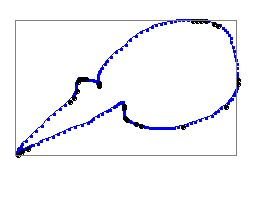
\includegraphics[scale=0.8]{images/stroke3.jpg.eps}
	\caption{Example of Input Stroke} Example of an input stroke to the system. 
	\label{fig:orignalStroke}
\end{figure}


\begin{figure}
	\centering
			\subfigure[ Speed Graph]{	\includegraphics[scale=0.5]{images/vel3orginal.png.eps}}
			\hfill
			\subfigure[ Time Difference Graph] {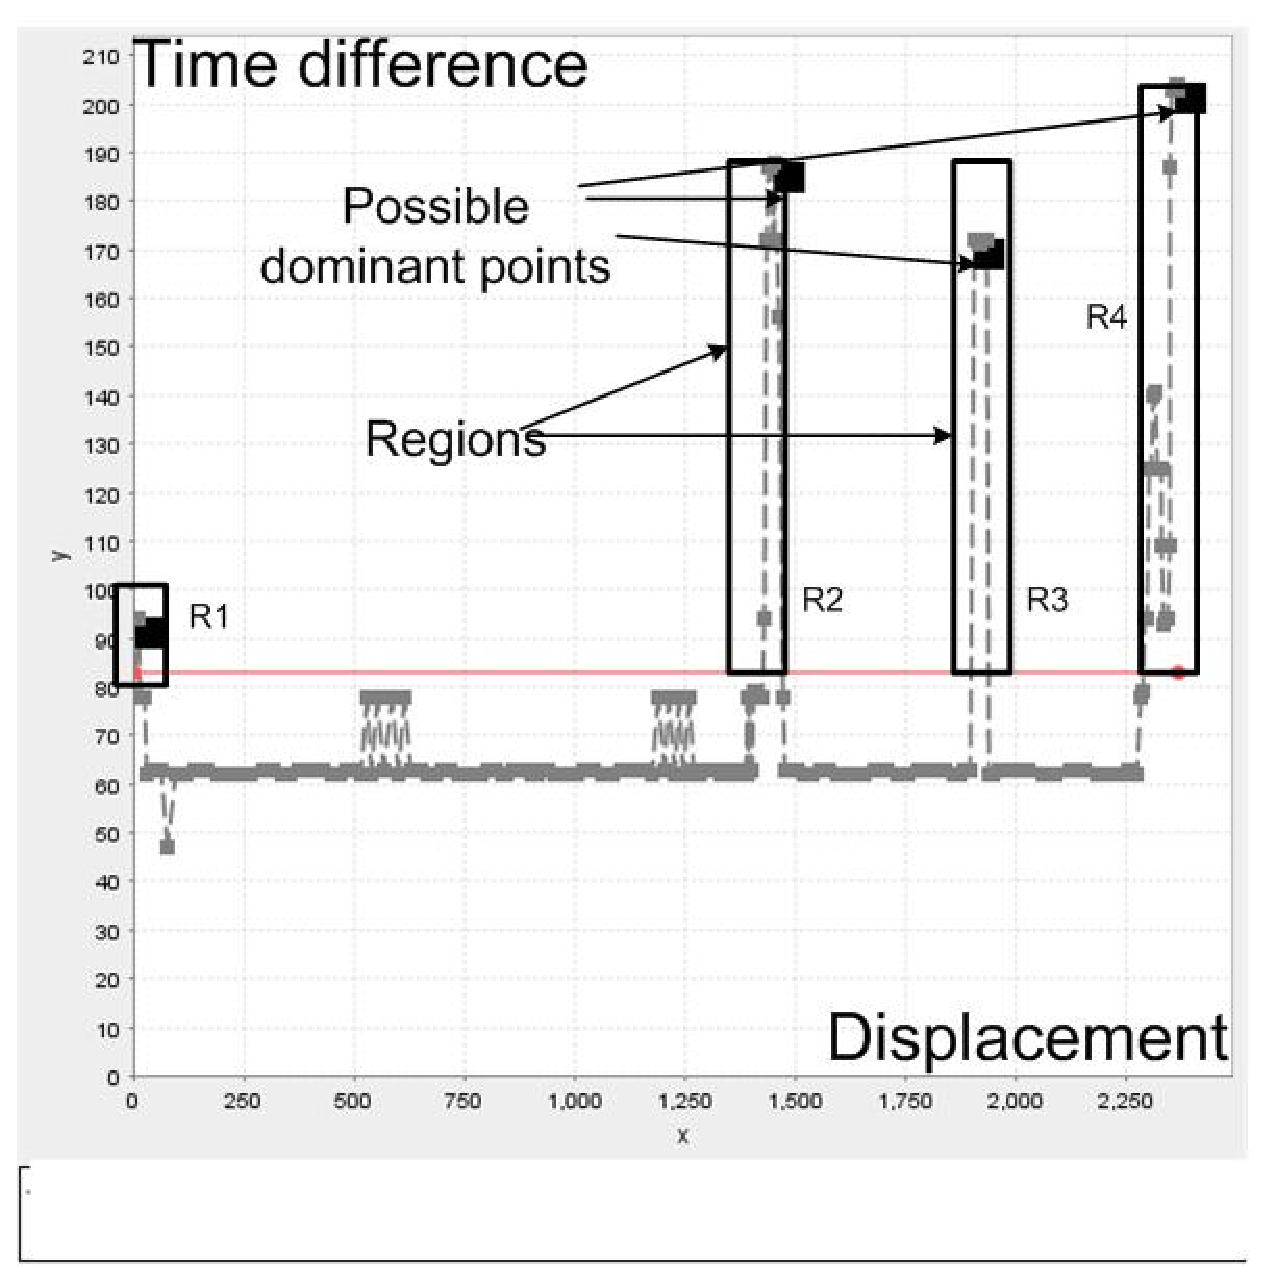
\includegraphics[scale=0.5]{images/td3.jpg.eps}}
	\caption{Speed and Time Difference Graphs}
	\label{fig:speed2Distance}
\end{figure}

\begin{figure}[]
	\centering
		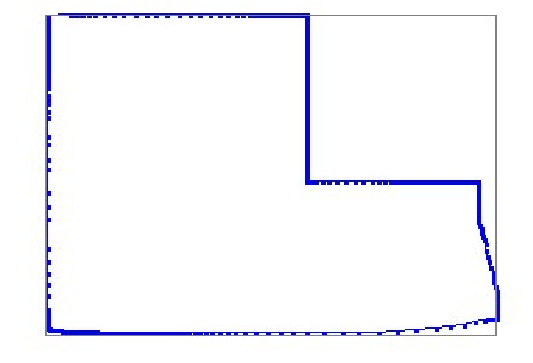
\includegraphics[scale=0.8]{images/orignalStroke.eps}
	\caption{Another Example of Input Stroke} Example of an input stroke to the system. 
	\label{fig:AnotherorignalStroke}
\end{figure}

\begin{figure}[]
%\begin{minipage}[b]{0.8\linewidth}
	\centering

	%	\subfigure[ The Speed of data] {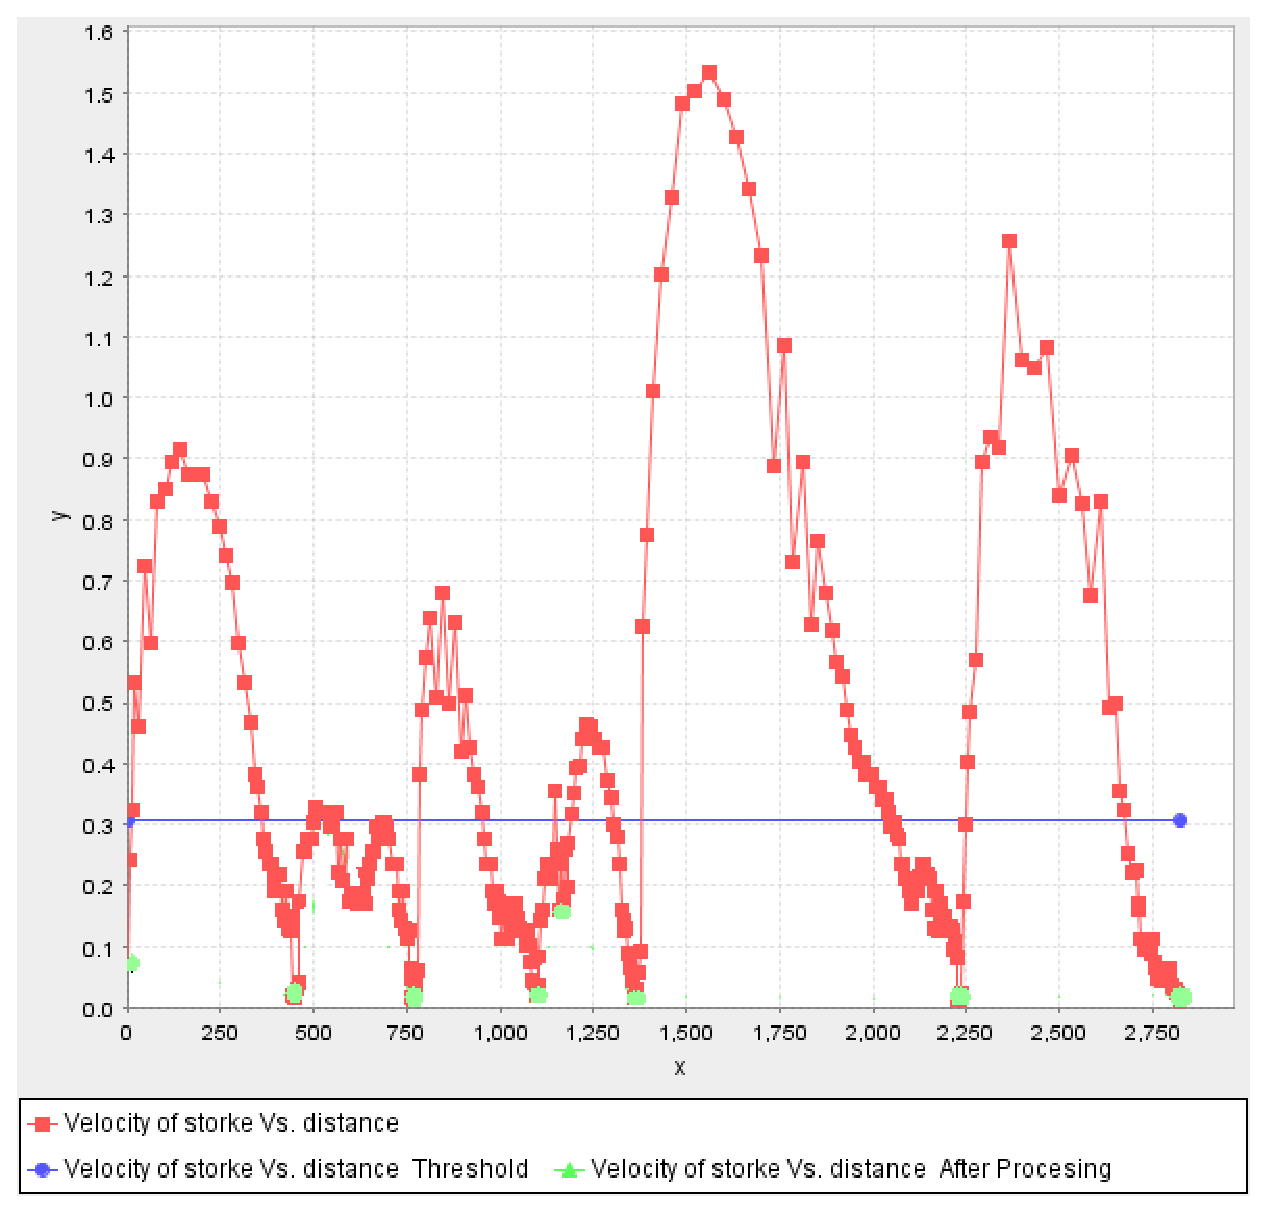
\includegraphics[scale=0.35]{images/speed2.eps}}
		
		\subfigure[ Direction Graph ] {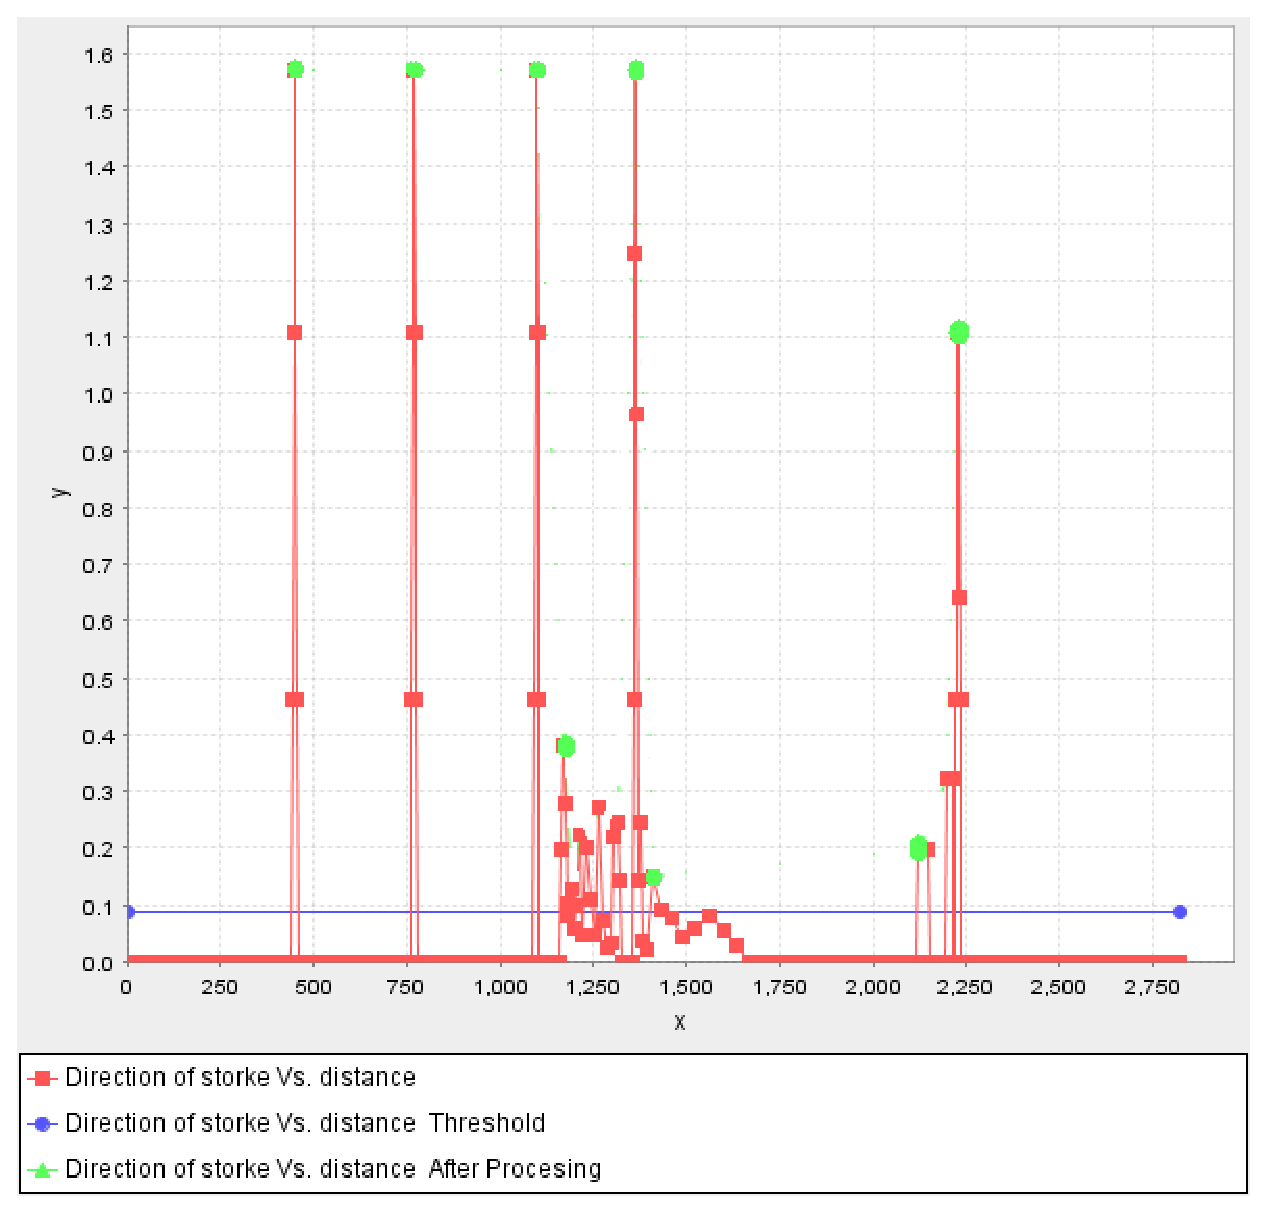
\includegraphics[scale=0.35]{images/direction2.eps}}
					%\end{minipage}
					%\begin{minipage}[b]{0.8\linewidth}
			\subfigure[Curvature Graph] {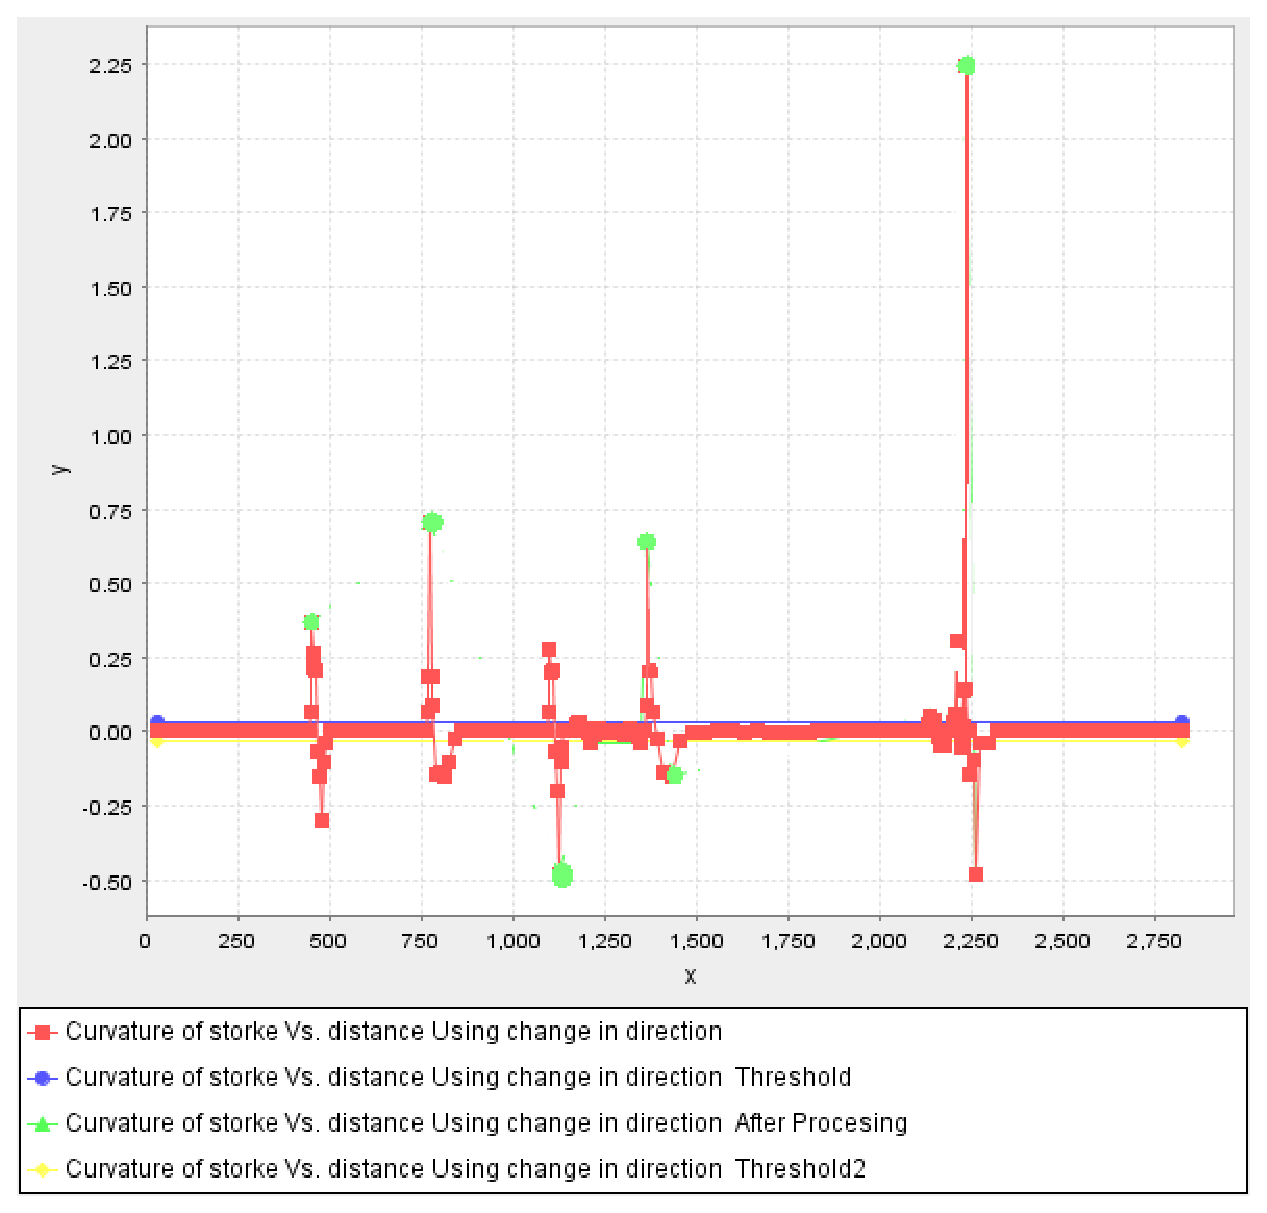
\includegraphics[scale=0.35]{images/curvature2.eps}}
		
			%\end{minipage}
	
	\caption{Curvature and Direction Graphs}%{The data of the stroke}
	
	\label{fig:curvatures}
\end{figure}


\subsection{Critical Point Detection}
\label{sec:CriticalPointDetection}
After computing speed, time difference and curvature information the system proceeds to detect the points with low velocity and high curvatures. Using simple differentiation to detect local extreme points resulted in false points due to the non smooth curves. Hence, the system adopted a process presented by \cite{earlyprocess}, where the mean of the curve is calculated. Then a threshold \textit{th} is used to separate the curve into regions; each region $Region_i$ is defined as a range of points, where the curve values are either above or below the threshold \textit{th}. Those regions are further processed to find the maximum point $Max(Region_i)$ of each region $Region_i$. The stroke points $p_i(x,y)$ that correspond to those maximum values are labeled as \textit{possible dominant points} $P_{pd}$. Figure \ref{fig:MaxRegioi} and \ref{fig:speed2Distance} shows an example of $Region_i$ of the speed curve and the dominant points $P_{pd}$ which correspond to the minimum of point in this region $Min(Region_i)$.  % (as shown are redundant)
\begin{figure}
	\centering
		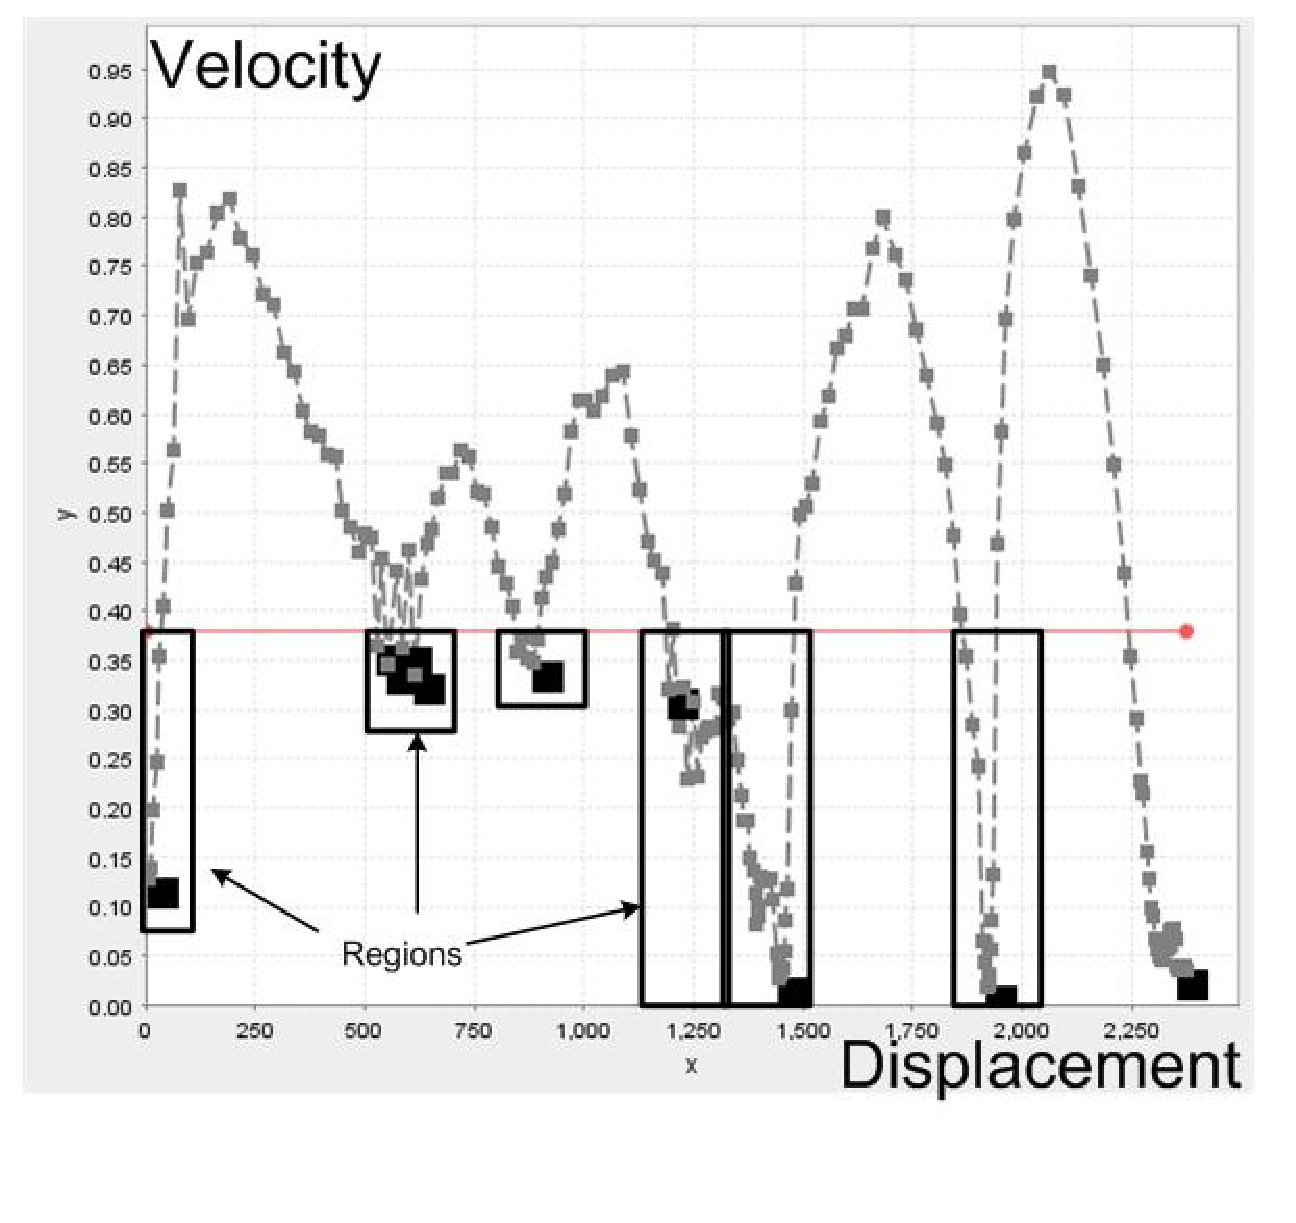
\includegraphics[scale=0.5]{images/vel3.jpg.eps}
	\caption{Possible Dominant Points Calculations}
	\label{fig:MaxRegioi}
\end{figure}

   %After the threshold is applied the curve is divided into regions. Each region is defined by a part in the data curve between tow intersection point of the threshold line and the curve.  % to find the extreme points. Hence, the mean of the direction curve is calculated and used as threshold.   \\
   %If we tried to differentiate the curve the result will be false threshold values we divide the data into regions of data higher or lower that the threshold. This will let us only look for high data only. The maximum of each region is then computed and reported as a possible vertex point. 
  
The system repeats this process to curvature, direction, time difference and speed curves. For each curve the points labeled as possible dominant points $P_{pd}$ are saved into a single array. The points that are repeatedly labeled are given a higher score than the other points. This score is then used to sort the  $P_{pd}$ points array. The array that contains possible points $P_{pd}$ is used as input for the next segmentation step. Figure \ref{fig:LabelsPPD} shows the particles labeled as Possible dominant points $P_{pd}$ by the Possible Dominant Point Extraction step, it is noticed the redundancy of some $P_{pd}$ points. 


\begin{figure}
	\centering
		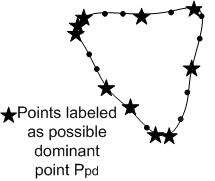
\includegraphics{images/ppd.eps}
	\caption{Possible dominant points}% a) Possible dominant point b) Particle encoding  
	\label{fig:LabelsPPD}
\end{figure}

\section{Segmentation}
\label{sec:Segmentation}
The segmentation tries to divide the stroke into a set of primitives. As shown in Figure \ref{fig:Blockdiagram} first an attempt is made to fit the stroke points into a curve or an ellipse using a minimum square error fitting algorithm \cite{chernov}. If the stroke proved to be an ellipse arc then the segmentation process ends and the system proceeds to the next step. Otherwise, the stroke is passed to two particle swarm algorithms that divide the stroke to either lines or lines and curves. The algorithms take the stroke points along with the possible dominant points $P_{pd}$ computed during Possible Dominant Point Extraction then produce a set of dominant points which are connected by either lines or curves. The next section describes the ellipse detection algorithm and the two particle swarm algorithms used to divide the stroke.
%If the stroke proved to be an ellipse then the segmentation process ends and the system proceeds to the next step. Otherwise, the stroke is passed into two particle swarm algorithms that will divide the stroke to either lines or lines and curves (see the block diagram in fig. \ref{fig:Blockdiagram} ). 
%The algorithms takes the stroke points along with the possible dominant points computed then produce a set of dominant points which are connected with either lines or curves (see fig. \ref{fig:Blockdiagram}).  The next sections will describe the ellipse detection algorithm and both the two particle swarm algorithms used to divide the stroke.
%After computing the primary data the system now tries \\
%Paragraphs describe the segmentation algorithm.  


\subsection{Ellipse Fitting }
\label{sec:EllipseDetection}

%The process starts by computing the center of the stroke bounding box. The bounding box center point is used as the first estimation of the ellipse center. The axes of the ellipse are estimated as $width/2$ and $height/2$ of the stroke bounding box. The least square fitting algorithm is used to minimize the fitting error of the ellipse equation \cite{chernov-2003}.  
This process tries to fit the stroke points into an ellipse arc; it starts with computing the center of the stroke bounding box. The bounding box center point is used as the first estimation of the center of the ellipse. The axes of the ellipse are estimated as the $width/2$ and $height/2$ of the stroke bounding box where $width$ is width and $height$ is height of the bonding box. The least square fitting algorithm \cite{chernov} is used to minimize the fitting error of the ellipse Equation (\ref{eq:circleFit})  

\begin{equation}
E = \sum\limits_{i = 0}^N {\frac{{(x_i - x_0 )}}{{a^2 }}^2  + \frac{{(y_i - y_0 )}}{{b^2 }}^2  - 1} 
\label{eq:circleFit}
\end{equation}

 where $N$ is number of points in the stroke, $a,b$ are the length of ellipse axes, $x_0$ \& $y_0$ are the coordinates of the center point, $x_i$ \& $y_i$ are the coordinates of point $i$ in the stroke. A list of new values for $x_0$ , $y_0$ ,$a$ and $b$ are generated randomly from the older values with small increments after each loop.  After few iteration, the final fit error of the estimated ellipse is reported. Another measure is used to compute the efficiency of the final estimated ellipse. Equation \ref{eq:circleError} ensures that the drawn percentage of ellipse is considered. This eliminates fitting a  line into very large ellipse but leaves small ellipses to be fitted as a partial or full ellipse. 


  \begin{equation}
eff = \left\{ {\begin{array}{*{20}c}
   {\frac{{P_{percent} }}{E}} & {ifP_{percent}  < 0.5}  \\
   {\frac{{P_{percent} }}{{E \times 2}}} & {ifP_{percent}  \ge 0.5}  \\
\end{array}} \right.
%eff= \begin{cases} 
% \frac{P_{percent}}{E},&\mbox{if} P_{percent}\mbox{< 0.5} \\
% \frac{P_{percent}}{2\times E},&\mbox{if} P_{percent}\mbox{\geq0.5} 
%\end{cases}
\label{eq:circleError}
\end{equation}
 \begin{equation}
P_{percent}  = L_{stroke} /P_{ellipse} 
\label{eq:ErrorArea}
\end{equation}
where $E$ is the error computed by Equation(\ref{eq:circleFit}), $L_{stroke}$ total length of stroke and $P_{ellipse}$ is the perimeter of the estimated ellipse. Figure \ref{fig:ellipseFitExamples} shows different $eff$, $P_{ellipse}$  and  $E$ values of strokes drawn by users.  If $eff$ is more than threshold $th_{Ellipse}$\footnote{By trial and error best threshold found was $th_{Ellipse}=0.25$} then the stroke is segmented as an ellipse otherwise the system proceeds to the next step. 

\begin{figure}
	\centering
		\includegraphics[scale=0.7]{images/ellipseFitError.eps}
	\caption{Ellipse Fitting Error}
	\label{fig:ellipseFitExamples}
\end{figure}


%Describe the ellipse detection algorithms 
%This process tries to fit the stroke points into an ellipse arc; it starts with computing the center of the stroke bounding box. The bounding box center point is used as the first estimation of the center of the ellipse. The axes of the ellipse are estimated as the $w/2$ and $h/2$ of the stroke bounding box where $w$ is width and $h$ is height of the bonding box. The least square fitting algorithm \cite{chernov-2003} is used to minimize the fitting error of the ellipse Equation (\ref{eq:circleFit})  
%
%\begin{equation}
%E = \sum\limits_{i = 0}^N {\frac{{(x_i - x_0 )}}{{a^2 }}^2  + \frac{{(y_i - y_0 )}}{{b^2 }}^2  - 1} 
%\label{eq:circleFit}
%\end{equation}
%
% where $N$ is number of points in the stroke, $a,b$ are the length of ellipse axes, $x_0$ \& $y_0$ are the coordinates of the center point, $x_i$ \& $y_i$ are the coordinates of point $i$ in the stroke. A list of new values for $x_0$ , $y_0$ ,$a$ and $b$ are generated randomly from the older values with small increments after each loop. After few loops, the final fit error and the ellipse confidence value are computed. The confidence value $Conf$ computed by Equation (\ref{eq:circleError})
% \begin{equation}
%Conf = E_{ellipse}+E_{area}
%\label{eq:circleError}
%\end{equation}
% \begin{equation}
%E_{area}  = \sqrt {\left( Area(stroke) - Area(ellipse)\right)^2 }
%\label{eq:ErrorArea}
%\end{equation}
%
%   where $E_{ellipse}$ is the error computed by Equation(\ref{eq:circleFit}) and $E_{area}$ is computed as the difference between the actual area of the stroke and the area of the estimated ellipse Equation(\ref{eq:ErrorArea}). If confidence value $Conf$ is less than threshold $th_{Ellipse}$\footnote{ Using trial and error the best threshold used is $th_{Ellipse}=0.7$ } the stroke is segmented as an ellipse otherwise the system proceeds to the two DPSO segmentation algorithms.  % The confidence value is used to label the stroke as ellipse or un segmented stroke. If the stroke as un-segmented the next process will be to pass the stroke into curve segmentation algorithm.    
   
 %  The next section describes the \textit{Discrete Particle Swarm Algorithm (DPSO)} then it proceeds to detail the two DPSO segmentation algorithms. 
   
   %to check if the stroke can be labeled as ellipse or not.\\ %is computed to check if stroke is an ellipse. \\
%We found that if the confidante is above threshold then the probability of ellipse is highest otherwise the stroke is passed to the next section to get the divisions of stroke and test its error.  


%\subsection{Discrete Particle Swarm Algorithm}
%\label{sec:ParticleSwarmAlgorithm}
%%\section{Particle Swarm Algorithm}
%%\label{PSO}
%%What is particle swarm algorithm and how it was used in related researches. 
%The main idea of \textit{Particle Swarm Algorithm (PSO)} is to represent each agent with a particle from the solution space \cite{PSOFirst}. Each agent moves the particle with a direction and velocity $v_{ij}$ based on equations \ref{eq:Swarm} \& \ref{eq:Swarm1}.
%\begin{equation}
%%\[
%p_{ij}=p_{ij}+v_{ij},
%%\
%\label{eq:Swarm1}
%\end{equation}
%where $p_{ij}$ represent the $jth$ particle in the $ith$ agent and $v_{ij}$ is the velocity of the $jth$ particle in the $ith$ agent.
% %Equation [\ref{eq:Swarm}] shows how velocity and direction of each particle are computed
% \begin{equation}
%v_{ij}  = v_{ij}  + c_1 r_1 (lbest_{ij}  - p_{ij} ) + c_2 r_2 (gbest_{ij}  - p_{ij} )
%\label{eq:Swarm}
%\end{equation}
% where $lbest_{ij}$ is the local best particle, $gbest_{ij}$ is the global best particle, $r_1$ \& $r_2$ are random variables and $c_1$ \& $c_2$ are the swarm system variables.
% After each iteration the global best $g_{best}$ particle and the agent local best $l_{best}$ particle are evaluated based on the maximum fitness functions of all particles in the solution space. The solution is found after achieving a specific number of iteration or after an error threshold is achieved.
%Equation \ref{eq:descrite}  
%\begin{equation}
%   P(i)\Leftarrow 
%\{
%\begin{array}{c} 
%1 \quad \quad if\quad r_{3}>p_{i}  \\
%
%0 \quad \quad if\quad r_{3}<p_{i} 
%\label{eq:descrite}
%\end{array}\}
%\end{equation}
% where $p_{ij}$ is the numerical values of the particle and $r_{3}$ is a random variable, is used to change the general swarm algorithm into binary particle (\textit{Discrete Particle Swarm Algorithm DPSO}) which handles particle values of either $0$ or $1$ \cite{PSODisceret}.  
\subsection{Non Ellipse Fitting}
\label{sec:SwarmSegmentation}
Two DPSO algorithms generate two different segmentations for each stroke. Each DPSO algorithms tries to find the best particle in the solution space. Both algorithms has the same problem formulation but different fitness functions. After generating two segmentations the system chooses the best segmentation from the outputs of the DPSO. The details of the problem formulation and fitness functions are given in the following sections.
%In this process the system generate two stroke segmentation using two PSO segmentation algorithm. The system generates segmentation from both algorithms and then chooses the segmentation with the minimum error value. The problem definition is the same in both algorithms but they differ in the fitness function and the error functions. %formation is nearly the same in both. 
\subsubsection{Problem Formulation}
\label{sec:ProblemFormulation}
The input stroke with $N$ points can be represented by set $S = \left\{ {x_1 ,x_2  \ldots x_N } \right\}$ where $x_i$ is the location of the point $i$ . The swarm algorithms consist of $M$ particles which are represented by the set 
$A  = \left\{ {P_i \left| {i = 1,2 \cdots M} \right.} \right\}$ where $P_i$ is a single solution particle from the solution space. Each particle decodes the problem with binary array with the same length $N$ as the input stroke (Figure \ref{fig:CodingSwarm}).   
\begin{figure}
	\centering
		\includegraphics{images/CodingSwarm.eps}
	\caption{An Example Stroke and the Coding}
	\label{fig:CodingSwarm}
\end{figure}
% The particles of the swarm represent a single solution of the solution space. For this problem the, each particle %will give a different segmentation for the input stroke. Firstly, we will define the stroke with N points by the set %S where.  We define the arc %An array with the same length as the number of points of the strokes.
The system represents each particle $P_i$ by $P_i = \left\{ {p_{ij} \left| {j = 1,2 \cdots N} \right.} \right\}$ where $p_{ij}$ is either 0 or 1 where $p_{ij}=1$ means that point $j$ is a dominant point(see Figure \ref{fig:CodingSwarm}.  Thus , the particle represents points that are chosen to be used as dominant points for this segmentation. 
The goal of the DPSO algorithm is to find the solution $P_i$ that generates the minimum set of dominant points that defines the stroke with minimum segmentation error. In other words, the system tries to find the fewer number of points (1's) location in the particle array which gives minimum segmentation error.  


The fitness function and error calculations are different in each algorithm. The first fitness and error function are described below. 

\subsubsection{Polygon Division Algorithm \textsl{AlgS1}}
\label{sec:PolygonDivisionAlgorithm}
The first algorithm, the algorithm tries to segment the stroke as a polygon. The final solution is a set of line segments that best define the input stroke. Given the inputs stroke let's define the set of points in the stroke as  $S = \left\{ {x_1 ,x_2  \ldots x_N } \right\}$ which is the set of consecutive points from start of stroke till the end. The arc $\widehat{x_ix_j}$ is defined as the consecutive set of points from point $x_i,x_{i+1} \cdots,x_j$. The line
$\overline{x_i x_j} $ is the straight line connecting point $x_i$ to point $x_j$. The approximation error is computed by the equation \ref{eq:ErrorSwarm1} 
\begin{equation}
E=\sum\nolimits_{i = 0}^M e ( \widehat{x_ix_{i+1}},\overline{x_i x_{i+1}})
\label{eq:ErrorSwarm1}
\end{equation}
 where $M$ is the number of dominant points in this solution.  The error $ e ( \widehat{x_ix_j},\overline{x_i x_j})$ is computed as the sum of squared perpendicular distance from every point along the arc $\widehat{x_ix_j}$ to the line $\overline{x_i x_j}$ \cite{PolygonApproximationPSO}. Figure \ref{fig:DPSOERROR} shows a graphical representation of the error. The fitness is computed using equation \ref{eq:fitnessSwarm1} 
\begin{equation}
\max fitness(p_i ) = \left\{ {\begin{array}{*{20}c}
   { - E/\varepsilon N} & {ifE > \varepsilon ,}  \\
   {D/\sum\limits_{j = 1}^N {p_{ij} } } & {otherwise}  \\
\end{array}} \right.
\label{eq:fitnessSwarm1}
\end{equation}%\]
where $N$ is the number of points in the stroke, $D$ is the number of point in the solution that was previously labeled as $P_{pd}$  and $E$ is the computed error and $\varepsilon$ is the error threshold which is computed as 20 \% of the input stroke area.  If the solution produced an error that exceed the error threshold $\varepsilon$ the fitness function assign a -ve value for the solution to express it's in feasibility, otherwise the inverse of the number of vertex produced is used to access the solution fitness in terms of minimum number of vertices'.   

This fitness function optimize two goals the first is to move the solution into the feasible solution space with acceptable error bounds and second is to fly the particle to a new position which may result in a polygon with a fewer number of vertices'\cite{PolygonApproximationPSO}.  The two optimization goals are pursued simultaneously since the DPSO evolves with swarm particles and each of which may invoke different fitness evaluation depending on the incurred approximation error. 
\begin{figure}
	\centering
  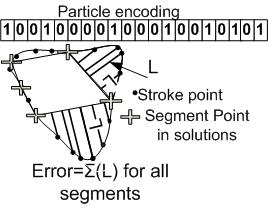
\includegraphics[scale=0.8]{images/pso1.eps}			
	\caption{AlgS1 Error}% a) Possible dominant point b) Particle encoding  
	\label{fig:DPSOERROR}
\end{figure}
 %The error is chosen to in favor of larger than the threshold is given a -ve value to lower the value of solution otherwise the system will favor the lower number of vertices'.\\ %we will want to lower the number of vertices'. \\
%if we say that s
%Alg1:sinc
%Alg2: 
\subsubsection{Hybrid Curve Algorithm \textsl{AlgS2}}
\label{sec:PolygonDivisionAlgorithm}

The second algorithm has the same problem formulation but different fitness and error functions. It was previously introduced in  \cite{CruveDivisionSwarm} where genetic programming was used as the optimizing algorithm. The particle is represented using the arrays $P_i = \left\{ {p_{ij} \left| {j = 1,2 \cdots N} \right.} \right\}$ where $p_{ij}$ is either 0 or 1. Lets denote the segments $\widehat{x_ix_j}$ as the consecutive set of points from point $x_i,x_{i+1} \cdots,x_j$. The algorithms attempts to fit each segment $\widehat{x_ix_j}$ to both line and circle. The type of the segment is determined according to the minimum error of each fit. The final error of the solutions is the summation of error of all segments.  %The goal of the algorithm is to fit the segments between the solution vertices' into straight lines or a circular arc. 
\paragraph{Fitting segments into straight line.}
\label{sec:FittingSegmentIntoStraightLine}
According to \cite{CruveDivisionSwarm} each segment $\widehat{x_ix_j}$ given a set of points $x_i,x_{i+1} \cdots,x_j$ can be fitted into the line: $y=kx+c$ where $k$ and $c$ are the slope and the intercept of the line respectively. Equation \ref{eq:Linek} and \ref{eq:LineC} 
\begin{equation}
\label{eq:Linek}
k = \frac{{N\sum\limits_{i = 1}^N {x_i y_i }  - \sum\limits_{i = 1}^N {x_i } \sum\limits_{i = 1}^N {y_i } }}{{N\sum\limits_{i = 1}^N {x_i^2 }  - \left( {\sum\limits_{i = 1}^N {x_i } } \right)^2 }}
\end{equation}
\begin{equation}
\label{eq:LineC}
c = \frac{{\sum\limits_{i = 1}^N {x_i^2 } \sum\limits_{i = 1}^N {y_i }  - \sum\limits_{i = 1}^N {x_i } \sum\limits_{i = 1}^N {x_i y_i } }}{{N\sum\limits_{i = 1}^N {x_i^2 }  - \left( {\sum\limits_{i = 1}^N {x_i } } \right)^2 }}
\end{equation}
, where $N$ is the number of points in the segment and $(x_i, y_i)$ are the coordinate of the point $i$, are used to fit the segment $\widehat{x_ix_j}$ into the straight line.
\begin{equation}
\label{eq:ds}
 d_s  = \frac{{\sum\limits_{i = 1}^N {\left| {(kx_i  + c) - y_i } \right|} }}{{N\sqrt {k^2  + 1} }}
\end{equation}
The distance ($d_s$) (Equation \ref{eq:ds}) is the average distance from segment points $(x_i, y_i)$ to the estimated line. This distance $d_s$ is used as the error of the line approximation.
\paragraph{Fitting segments into circular arc.}
\label{sec:FittingSegmentcirculararc}
Each segment is also fitted into a circular arc $(x - a)^2  + (y - b)^2  = R^2, $ where ($a,b$) are the coordinate of the center of the circle and $R$ is the radius of the circle. They is estimated using the following set of equations: 
 
\begin{equation}
a = \frac{{b_{1}a_{22} - b_{2}a_{12}}}{\Delta},
\end{equation}
\begin{equation}
	b = \frac{{b_{2}a_{11} - b_{1}a_{21}}}{\Delta},
\end{equation}
\begin{equation}
R = \sqrt {\frac{1}{N}(\sum\limits_{i = 1}^N {x_i^2 }  - 2\sum\limits_{i = 1}^N {x_i a}  + Na^2  + \sum\limits_{i = 1}^N {y_i^2  - 2} \sum\limits_{i = 1}^N {y_i b + Nb^2 } )} ,
\end{equation}

Where 
\begin{equation}
a_{11}  = 2\left[ {\left( {\sum\limits_{i = 1}^N {x_i } } \right) - N\sum\limits_{i = 1}^N {x_i^2 } } \right]
\end{equation}
\begin{equation}
a_{12}  = a_{21}  = 2\left( {\sum\limits_{i = 1}^N {x_i \sum\limits_{i = 1}^N {y_i } }  - N\sum\limits_{i = 1}^N {x_i y_i^2 } } \right),
\end{equation}
\begin{equation}
 a_{22}  = 2\left[ {\left( {\sum\limits_{i = 0}^N {y_i } } \right)^2  - N\sum\limits_{i = 0}^N {y_i^2 } } \right]
\end{equation}
\begin{equation}
b_1  = \sum\limits_{i = 0}^N {x_i^2 } \sum\limits_{i = 0}^N {x_i }  - N\sum\limits_{i = 0}^N {x_i^3 }  + \sum\limits_{i = 0}^N {x_i } \sum\limits_{i = 0}^N {y_i^2 }  - N\sum\limits_{i = 0}^N {x_i y_i^2 } , 
\end{equation}
\begin{equation}
b_2  = \sum\limits_{i = 0}^N {x_i^2 } \sum\limits_{i = 0}^N {y_i }  - N\sum\limits_{i = 0}^N {y_i^3 }  + \sum\limits_{i = 0}^N {y_i } \sum\limits_{i = 0}^N {y_i^2 }  - N\sum\limits_{i = 0}^N {x_i^2 y_i } ,
\end{equation}

\begin{equation}
\Delta  = a_{11}b_{22}-a_{12}a_{21}.
\end{equation}
 The error of the circle estimation is measured using the distance $d_c$ which is calculated using equation \ref{eq:circleE}:
 \begin{equation}
 \label{eq:circleE}
d_c  = \frac{{\sum\limits_{i = 0}^N {\left| {\sqrt {(x_i  - a)^2  + (y_i  - b)^2 }  - R} \right|} }}{N}
\end{equation}
Thus, Equation \ref{eq:circleE} $d_c$ defines the average distance $d_c$ from the segment points $x_i,y_i$ to the estimated circle ($a,b$) and $R$.

\paragraph{Determining The Segment Type.} 
\label{sec:DeterminigSegmentType}
If the average distance $d_s$ equals zero this means that the segment$\widehat{x_ix_j}$ points is exactly the straight line approximated. If the distance ($d_c$) equals zero means that the segments point lies exactly on the circular arc estimated. But the user rarely draws an exact line or circle, so the distances are used as the fitting error. The minimum distance determines the type of the current segment, in other words if ($d_s$) is smaller than ($d_c$) then the segment is labeled as a line segment otherwise it is labeled as a circular arc. 


After each segment type is determined the particle segmentation error is computed by Equation \ref{eq:errorSwarm2} 
\begin{equation}
E=\sum\nolimits_{i = 0}^M e(D_i) 
\label{eq:errorSwarm2}
\end{equation}
where $M$ is the number of segments in the solution, $D_i$ is the  approximation error of each segment as $min(d_c,d_s)$ as computed in Equation\ref{eq:circleE}  and Equation \ref{eq:ds} \cite{CruveDivisionSwarm}. The fitness is computed by the equation \ref{eq:fitnessSwarm2} 
\begin{equation}
\max fitness(P_i ) = \frac{1}{{E \times M^k }}
\label{eq:fitnessSwarm2}
\end{equation} where $E$ is the error and $M$ is number of segments and $k$ is a parameter tweaked to get minimum number of segments. $k$ is selected to be 0.5\cite{CruveDivisionSwarm}. 

\subsubsection{Solution Refine procedures} 
%\cite{PolygonApproximationPSO} used a merge and divide algorithm after each loop of the swarm system to refine the solution but we used another enhancement method.
 After each loop in the swarm algorithm, each particle loops on the set of selected dominant points to enhance the solution. Each dominant point is checked to find if it was labeled before as a possible dominant (computed as in section \ref{sec:Preprocessing}), if not the point is moved to the nearest labeled point.
   After each loop of the swarm algorithm (\textsl{AlgS1} and \textsl{AlgS2}), each particle is refined using the following procedure. For each particle $P_i$ each dominant point $P_{ij}$ is checked to find if it was labeled before as a \textit{possible dominant point} $P_{pd}$ (computed as in section \ref{sec:Preprocessing}). If it was not labeled the point $P_{ij}$ is moved to the nearest labeled point. This ensures that all of the points generated by the DPSO are possible dominant points $P_{pd}$. After that the particles are tested to make sure that the distance between every two successive dominant point is larger than the constant $min_D$. If two points are nearer than $min_D$\footnote{ 5\% of the total stroke length} then one of the points is removed. 
   
\subsection{Choosing the Best Fit}
\label{sec:bestFit}
The two PSO algorithms produce two segmentation solutions. After that the system evaluates each solution to finally select the best segmentation. This evaluation is based on the area of both the segmentation and the input stroke. The segmentation error($E_{alg}$ )represents the sum of Square Root Error of the length from the point on the stroke to the estimated curve or line. In \textsl{AlgS2}, this error is the same as the computed error in Equation \ref{eq:ErrorSwarm1} but For the second algorithm \textsl{AlgS2} it is different than the computed error in Equation \ref{eq:errorSwarm2}. The additional computation is necessary to  compare the two segmentation fairly. The system choose the minimum segmentation as the final segmentation of this stroke. 


After the best fit segmentation is chosen the parameter of each primitive is computed. For example, if the stroke is represented as an ellipse, the center and axis of the ellipse is computed and confirmed. For lines the slope, equation, start point and end point are computed.  These values and parameter will help determine the spatial relations between different segments in the feature extraction step. 
% The segmentation which crossponds to the minimum $E_{tot}$ is the best segmentation.  
%\begin{equation}
%\label{eq:bestFit1}
%E_{area}=A_{st}-A_{sg}
% \end{equation}
% \begin{equation}
% where $A_{st}$ is the area of the input stroke, $A_{sg}$ is area of computed segmentation, $E_{alg}$ is the Segmentation Error. 
  
\section{Hybrid Segmentation Algorithm \textsl{Alg3}}
\label{sec:BenchMarckAlgorithm}

In this research, we developed another algorithm as reference to the results obtained by the DPSO algorithms. The algorithm was first implemented by  Sezgin et al. in \cite{earlyprocess}. The algorithm is divided into the following steps: 
\begin{enumerate}
	\item Compute the curvature and the speed for each point in the stroke. 
	\item   A percentage of maximum value of the speed and curvature is used as threshold.
		\item Mark the values higher than the threshold in a new arrays $L_c$ as the list of corner points generated from the curvature curve. The list $L_s$ contains the points generated from the speed curve.
	\item Compute a confidence on each list based on the type of curve. Then sort the lists $L_s$and $L_c$ by the confidence value. 
	\item Find the intersection points in both list and generate the a Sample solution $h_{curr}$. 
	\item Use $h_{curr}$ as initial solution. Loop on the following:
	
		\begin{enumerate}
			\item Generate a new solution $h_{s}$ using $h_{curr}$ and  the first point in the $L_s$ list .
			\item Generate a new solution $h_{c}$ using $h_{curr}$ and  the first point in the $L_c$ list.
			\item Test the solutions $h_{s},h_c$ to find the minimum solution.
			\item  If $h_s$ is the minimum then add the solution a list of hybrid solutions $Solutions_{set}$ and remove the first point from the list $L_s$ then set $h_s$ as $h_{curr}$. 
			\item If $h_c$ then add the solution a list of hybrid solutions $Solutions_{set}$ and remove the first point from the list $L_c$ then set $h_c$ as $h_{curr}$. 
		\end{enumerate}
		\item Choose the final solution from the list of solutions $Solutions_{set}$ as a tradeoff between  minimum error and number of corners.  
		\item Check each segment in the solution if the solution is can be estimated as a line segment if not it is fitted using a higher level Bezire curve. 
\end{enumerate}
More details about the algorithm are in \cite{earlyprocess}.


%\section{Stroke Clustring Algorithms }
%\label{sec:ClustringAlgoirthm}
%
%When the user finishes drawing a stroke the segmentation algorithm generate a list of segments that represent this stroke. The system then groups the segments generated from the segmentation algorithm. %These segments are grouped into a symbol and tested if they can be classified into one of the known symbols. If no identification is achieved the segments are added into a list of unclassified segments. When a user draws another stroke the segmented stroke is added to the list and the process is repeated until all the segments are classified to a known symbol.\\
%
%After the user draw all strokes of the symbol he has to wait 10 seconds or press finish button beside the drawing area. The set of unrecognized strokes is grouped together along with their segmentation as input to the feature extraction process. 

\section{Feature Extraction Methods}%%Feature Set
\label{sec:FeatureExtraction}

After the segmentation, each stroke is represented as a list of segments $L_s$. A segment can be either an ellipse, a line or a circular arc. The list of segments $L_s$ represents the segmentation of the stroke. When a user draw another stroke the generated segmentation of the stroke is appended to the list of segments.  When the user finish drawing the symbol the segment list $L_s$ will contain all segments of the drawn symbol. The relation and properties between different segments are extracted from the segment list $L_s$.  This step is considered as feature extraction which is described in details in the next sections. 

The system uses a composite set of features (total of 70 features) which include global shape properties like Rubine feature set \cite{gestureexample12},  ink density \cite{GeometryAndDomain102}, some appearance based properties like Zernike moments \cite{HeloiseBeautification}, and some stroke based structural information like number of perpendiculars lines , number of parallel lines and types of primitives in each symbol. The following list gives details on all the features used in the system.


\subsection{Structural and geometrical Features(FS1)}
 Features defines the structure of the geometrical symbol. Section \ref{sec:steprec} describe in details how these 13 feature are computed.  
%\begin{description}
% \item [Structural and geometrical Features (FS1)] 
  \begin{itemize}
	 \item \emph{Segments:} Number of segments in the symbol.
	 \item \emph{Strokes:} Number of strokes or partial strokes that created the symbols.  
		\item  \emph{Primitives:} Number of primitives in the symbol. The feature helps when identifying             symbols with mixed geometric primitives like cylinders and callouts.  
		\item \emph{Curves:} Number of curves or ellipses in the symbol. 
		\item \emph{Lines:} Number of lines in the symbol. 
		\item \emph{Perpendicular} lines Number of perpendicular lines. 
		\item \emph{Parallel} lines Number of parallel lines. 
		\item \emph{Intersections} Number of intersection between lines and curves. 
		\item \emph{T intersections} Number of T intersections. 
		\item \emph{L intersections} Number of L intersections. 
		\item \emph{X intersections} Number of X intersections.
		\item \emph{Min Radius} Minimum Radius of all curves in the symbol.
		\item \emph{Max Radius} Maximum Radius of all curves in the symbol.
		%\item[No. of holes] Number of holes in the symbols. 
\end{itemize}
%\begin{description}
%	 \item[Segments] Number of segments in the symbol.
%	 \item [Strokes] Number of strokes or partial strokes that created the symbols.  
%		\item[Primitives] Number of primitives in the symbol. The feature helps when identifying             symbols with mixed geometric primitives like cylinders and callouts.  
%		\item [Curves] Number of curves or ellipses in the symbol. 
%		\item [Lines] Number of lines in the symbol. 
%		\item [Perpendicular lines] Number of perpendicular lines. 
%		\item [Parallel lines] Number of parallel lines. 
%		\item [Intersections] Number of intersection between lines and curves. 
%		\item [T intersections] Number of T intersections. 
%		\item [L intersections] Number of L intersections. 
%		\item [X intersections] Number of X intersections.
%		
%		
%		%\item[No. of holes] Number of holes in the symbols. 
%
%\end{description}
\subsection{Rubine Feature Set (FS2)} Features introduced by Rubine\cite{gestureexample12} for single stroke gestures. These 12 features represent the global shape of the symbol drawn. To compute the features we append all segments points into single path $ink_{path}$. The features is computed on the generated path $ink_{path}$.%then compute the features based on this path.  
\begin{enumerate}
	\item Cosine of starting angle.
	\item Sine of starting angle.
	\item Length of diagonal of bounding box. It gives an idea of the size of the bounding box).
	\item Angle of diagonal. It gives an idea of the shape of the bounding box (long, tall, square).
	\item Distance from start to end.  
	\item Total stroke length
	\item Change in Rotation( Arctan ). It gives the directional angle.
	\item Absolute rotation 
	\item Rotation squared 
	\item The maximum speed reached (squared) 
	\item Total time of stroke 
\end{enumerate}
\subsection{Statistical Features (FS3)} 
\begin{enumerate}
	\item \textsl{Zernike moments:} Zernike moments of order $n$\footnote{ We tried different values of n. Results show the analysis of each order.} \cite{HeloiseBeautification}.  For $n=10$ there are 32 moment features. 
\end{enumerate}
\subsection{Global shape properties set (FS4)}
 Features that are composites of different geometrical and statistical symbol. These 13 features represent the global shape of the symbol drawn.

 	\begin{itemize}
\item \emph{Size Ratio} Ratio between width to height of the symbol.
		\item \emph{Log of size Ratio} Log of the ratio between width and height of symbol.
	\item \emph{Ink density} Compute the density of points inside its bounding box\cite{GeometryAndDomain102}.   
 	\item \emph{Convex Hull Area} Area of convex hull with respect to area of bounding box of symbol.
  
	\item \emph{Convex Hull Perimeter} Perimeter of convex hull with respect to total length of symbol.
		\item \emph{Convex Hull Point} Number of points of convex hull with respect to Number of points of symbol.
		\item \emph{Mean Centroidal radius} The Mean of the centroidal radius which is the distance from each point in the symbol to the center of gravity.
				\item \emph{Center of Gravity} The center of gravity of the symbol (both in y and x direction).
					\item \emph{Mean Time} The mean of the time values between each two successive points in the symbol. %Different strokes are appended to construct a single path.
	%\item [Ra]	
				
	\item \emph{Mean Time difference} The mean of the time difference between each two successive points in the symbol. %Different strokes are appended to construct a single path.
	%\item [Ra]		
			\item \emph{Log of Area} Log of area of the symbol.
	\item \emph{Diff Area} Absolute difference of the area of bounding box and area of symbol.
	
  \end{itemize}
  
 Section \ref{sec:featuresComparisions} presents a comparative result of the different feature sets from these features.

\section{Classification}%%Feature Set
\label{sec:Classification}
The system uses support vector machine (SVM) classifier with Linear kernel (Linear kernel) \cite{libsvm}. SVM is a binary classifier that maximizes the margin between the decision boundary and the support vectors. To enable SVM to learn multi classes we used one versus one strategy for combining set of binary classifier. This strategy trains $ \frac{n(n-1)}{{2}}$ binary classifier each distinguish between only two shapes. The final result is based on a number of votes each shape has from all classifiers. We used the library implementation of LibSVM \cite{libsvm} and its implementation of the one-vs-one strategy. Section \ref{Sec:SVMdetail} describe in details the classifier, how classes (classification) are determined and the reasons behind using this specific classification methods.

\subsection {Training and Testing}
A training set that contains positive samples of each category in the data set is used to train the SVM classifier.  The training starts after computing the feature vector of each sample. The system trains $ \frac{n(n-1)}{{2}}$ binary classifiers each distinguish between only two categories. The goal of the training process is to generate a linear SVM plane that maximize margin between the two categories.  A cross validation procedure is implemented to choose the best value for the $C$ parameter in SVM classifier.( $C=100$ was the best value) 
=
For classification the decision is made from producing the feature vector of the unknown symbol to the trained $\frac{n(n-1)}{{2}}$ binary classifiers. The final decision is given using simple voting strategy. 



\subsection{Support Vector Machines}
\label{Sec:SVMdetail}
The foundation of Support Vector Machines (SVM) were developed by Vapnik \cite{svmintroduce} in 1995. It is gaining increase popularity due to the high performance and efficient implementation. The goal of SVM algorithms is to generate a separating plane between two different classes which are represented using a set of n-dimensional vectors. The generated plane is used as a good classifier to the unseen examples. However, there can be more than one plane that can separates the data therefore SVM attempts to find the plane that maximize the margin (distance between classifier and nearest sample) between the two classes \ref{fig:svm1}. To calculate the margin, two different hyper planes are constructed, one plane on each side of the data, these two planes are then moved to generate the maximum margin possible.  
\begin{figure}
	\centering
		\includegraphics{afterDefense/svm1.jpg.eps}
	\caption{Different Classifier Planes }
	\label{fig:svm1}
\end{figure}


Let us consider a two class classification task with data points $x_i$ where $i=1,\cdots,m$ having corresponding labels $y_i=\pm1$ where if  $y_i=1$ if $x_i$ belonged to first class and $y_i=-1$ if $x_i$ belonged to second class. Each data point $x_i$ is represented in $N$ dimensional input or attribute space. Let the classification plane be represented as function. 
\begin{equation}
 y=f(x)=sign(\omega \cdot x - b)
\label{eq:planeEq}
\end{equation}

 The orientation of the separation plane is determined using the vector $\omega$ and the offset of the plane from the origin is determined using the scalar $b$.   Let's make an assumption that the data point are linearly separable, i.e. there are infinite possibilities to find a plane that separates and correctly classify the training data. This is idea is illustrated in Figure\ref{fig:svm1} where two different separating planes can correctly classify the data. It is intuitively noted from the figure that the solid line is more likely to generalize more data. This means less classification error will be introduced. The geometrical characterization of this plane means the plane furthest from both classes.     % Which one is preferable ? Intuitively one prefers the solid pane since small perturbations of any point would not introduce misclassifications errors. Without any information, the solid plane is more likely to generalize better on future data. Geometrically we can characterize the solid plane as being furtherer from both classes.  Plane supports a class if all points in that class are on one side of that plane.
 
The main problem of SVM is constructing the plane that is furthest from both classes. The main approach is to use two parallel supporting planes and maximize the margin between them. All point in a class should be in one side of the plane in order to be a supporting plane.  Therefore, for the points with the class label $+1$ we would like there exist $\omega$ and $b$ such that $\omega \cdot x_i\> b$ or $\omega \cdot x_i -b \> 0$%, and for the points with class label $-1$ we would like there exist $\omega$ and $b$ such that $\omega \cdot x_i \< b $.
Suppose that smallest value of $\mid \omega \cdot x_i -b\mid$ is $\kappa$, then when $ \omega \cdot x_i -b \geq \kappa$. The argument inside the decision function is invariant under positive rescaling so we will implicitly fix a scale by requiring $\omega \cdot x_i -b \geq 1 $. Similarly the points with class label $-1$ requires $\omega \cdot x_i -b \leq -1 $. To find the plane furthest from both classes, we need to maximize the distance between the support planes for each class as illustrated in Figure \ref{fig:svm2}. To accomplish this, both planes are pushed apart until they bump into small number of data points ( the support vectors ) for each class. Figure \ref{fig:svm2} shows the support vectors as filled data points, 
\begin{figure}
	\centering
		\includegraphics{afterDefense/svm2.jpg.eps}
	\caption{Margin of SVM Support planes }
	\label{fig:svm2}
\end{figure}


The distance between these supporting planes 
\begin{equation}
 \omega \cdot x=b+1 \\
  \omega \cdot x=b-1
\end{equation}
is 
\begin{equation}
 \gamma = \frac{2}{\parallel \omega \parallel^2}
\end{equation}

Thus maximizing the margin is equivalent to minimizing $\frac{{\parallel \omega \parallel}^2}{2}$ in the next quadratic program 

\begin{equation}
 \min_{\omega,b}  \frac{{\parallel \omega \parallel}^2}{2}
\end{equation}
\begin{equation}	
\begin{array}{cc}
 s.t. \ \ \   \omega \cdot x_i \geq b+1 &    y_i \in Class 1 \\ 
 \ \ \ \ \ \   \omega \cdot x_i \leq b-1 &    y_i \in Class -1 
  \end{array} 
\end{equation}

The constrain can be simplified to $y_i(\omega \cdot x_i-b)\geq 1$. 

The Support vectors that are pumped into the supporting plane determine the margin. This is a primal form Quadratic Programming (QP) problem. The concept of duality can also used to wields the problem to a Largrnigian dual QP problem in Equation \ref{eq:dual}. 
% maximum margin between parallel 
\begin{equation}
\begin{array}{c}
\min_{\alpha} \ \ \   \frac{1}{2} \sum_{i=1}^{m}{\sum_{j=1}^{m}{y_iy_j\alpha_i\alpha_jx_ix_j}} - \sum_{i=1}^{m}{\alpha_i} \\
s.t. \ \ \sum_{i=1}^{m}{y_i\alpha_i}=0   \\
  \alpha_i \geq 0  \ \ \ i=1,\cdots , m 
  \end{array} 
\label{eq:dual}
\end{equation}

Both the dual form and the primal form wields to the same plane $\omega=\sum_{i=1}^{m}y_i\alpha_i x_i$ and threshold $b$ determined by the support vectors (for which $\alpha_i\geq 0$). 

\subsubsection{Theoretical foundation}

The generalization error on future points and not only in the training set can be obtained as proved by the statistical learning theory \cite{BennettSVMP2000}.  The generalized error bound is a function of the misclassified error on the training data and the terms that measure the complexity or capacity of the classification. In linear functions, using planes to maximize the margin of separation reduces the complexity of the functions. Thus, by explicitly maximizing the margin we are in the same time minimizing bound on the generalization error and therefore expect better generalization with high probability. The dimensionality of the data does not affect the size of the margin which   results in good performance for very high dimensional data (i.e, with a very large number of attribute). In a sense, this also reduces the problems caused by over fitting of high - dimensional data.  A large volume of literature, e.g., \cite{bookSVMoverfit11,statisticalSVM1} refers to this problem,  for more technical discussion of the   statistical theory. 

%Using geometric arguments we can gain insights to some of these results. Classification function that have capacity to fit the training data are more likely to over fit resulting in poor generalization.  

\subsubsection{Linearly Inseparable Case}
In all previous sections we assumed that the problem of classifying two set is linearly separable. The assumption is not true in most cases, thus, trying to construct a plane to separate the two dataset will fail. Figure \ref{fig:svm5} illustrates that we cannot construct a plane that can separate the two sets correctly. The constrains for constructing the planes must be relaxed since the QP task is not feasible for the linearly inseparable case.  Consider the linear inseparable problem in Figure\ref{fig:svm5}, in the ideal case there will be no point misclassified and no point falls on the margin. But we must relax the constrain that insure that each point in on the appropriate side of it is supporting plane. Every point that falls on the wrong side of the supporting plane is considered an error. The problem is now to maximize the margin and minimize the error.  
 
\begin{figure}
	\centering
		\includegraphics{afterDefense/svm5.jpg.eps}
	\caption{Example of SVM Linearly Inseparable Problem}
	\label{fig:svm5}
\end{figure}
A minor change in the supporting plane QP problem can accomplish this. A non negative slack or error variable $z_i$ is added to each constraint.  A weighted penalty term is also added to the objective as follows:
 \begin{equation}
 \begin{array}{c}
\min_{w,b,z}  \quad \frac{{\parallel \omega \parallel}^2}{2}+C \sum_{i=1}^{l}z_i  \\
s.t.  \quad y_i(\omega \cdot x_i -b)+z_i \geq 1  \\
    z_i \geq 0  i=1,\cdots,m
\end{array} 
\label{eq:inseperable}
\end{equation} 

The primal relaxed supporting plane method is equivalent to the dual problem. The Largangian dual of the QP task is :

\begin{equation}
\begin{array}{c}
\min_{\alpha} \ \ \   \frac{1}{2} \sum_{i=1}^{m}{\sum_{j=1}^{m}{y_iy_j\alpha_i\alpha_jx_ix_j}} - \sum_{i=1}^{m}{\alpha_i} \\
s.t. \ \ \sum_{i=1}^{m}{y_i\alpha_i}=0   \\
 C \geq \alpha_i \geq 0  \ \ \ i=1,\cdots , m 
 \end{array} 
\label{eq:dual}
\end{equation}



\subsubsection {Non linear function Using Kernels}
Figure \ref{fig:svm6} shows a classification problem that cannot be separated using linear space. A higher order plane can work better in similar cases. Converting a linear classification algorithm into non linear classification algorithm can be achieved by adding additional attribute to the data that are nonlinear functions of the original data. The expanded dataset features space can be separated using an existing linear classification algorithm.  The linear classification that is applied on the feature space produces a non linear classification on the original input space. In two dimensional vector space with attributes $r$ and $s$, to construct a quadratic  discriminate  simply map the original two dimensional input space $\left[r,s\right]$ to  five dimensional features space $\left[r,s,rs,r^2,s^2\right]$ and construct a linear discriminate in that space. specifically, define : $\vartheta(x):R^2  \rightarrow R^5$ then 
\begin{equation}
\begin{array}{l}
	x=[r,s] \\
	\omega \cdot x=\omega_1 r+ \omega_2 s \\
	\downarrow \\
	\vartheta(x)=\left[r,s,rs,r^2,s^2\right] \\
	
	 \omega \cdot \vartheta(x)= \omega_1 r+ \omega_2 s + \omega_3 rs+ \omega_4 r^2+\omega_5 r^2 
\end{array}
\label{eq:kernel}
\end{equation}  

The resulting classification function, 
\begin{equation}
\begin{array}{l}
f(x)=sign\left( \omega \cdot\vartheta(x)-b \right) \\
= sign\left( \omega_1 r+ \omega_2 s + \omega_3 rs+ \omega_4 r^2+\omega_5 r^2 -b \right) 
\end{array}
\label{eq:kern2}
\end{equation}  
is linear in the mapped five dimensional feature space but is quadratic in the two dimensional input space. 

\begin{figure}
	\centering
		\includegraphics{afterDefense/svm6.jpg.eps}
	\caption{Example of an non Linearly SVM Problem }
	\label{fig:svm6}
\end{figure}

For higher dimensional datasets, this method of nonlinear mapping has two potential problems stemming from the fact that dimensionality of the feature space explodes exponentially. The first problem is that over fitting becomes a problem. However, since SVM rely on margin maximization they are largely immune to this problem. Provided an appropriate value of parameter $C$ is chosen. The second concern is that it is the computational complexity of   computing $\vartheta(x)$ but SVM use kernels to get around this problem.  

Examine what happens when  the nonlinear mapping is introduced to equation \ref{eq:dual}. Let us define: $\vartheta(x):R^2\rightarrow R^5 \quad n>> n$  we need to optimize

\begin{equation}
\begin{array}{c}
\min_{\alpha} \ \ \   \frac{1}{2} \sum_{i=1}^{m}{\sum_{j=1}^{m}{y_iy_j\alpha_i\alpha_j\vartheta(x_i)\vartheta(x_j)}} - \sum_{i=1}^{m}{\alpha_i} \\
s.t. \ \ \sum_{i=1}^{m}{y_i\alpha_i}=0   \\
 C \geq \alpha_i \geq 0  \ \ \ i=1,\cdots , m 
 \end{array} 
\label{eq:dualkernel}
\end{equation}
Notice that the mapped data only occurs as inner product in the objective. Now we apply a little mathematically magic known as Hilbert Schmidt kernels, first applied to SVM in \cite{svmintroduce}.  By Mercer's theorem, we know that for certain mapping $\theta$ and any two points $u$ and $v$, the inner product of the mapped points can be evaluated using the kernel function without ever explicitly knowing the mapping, e.g., $\theta(u)\theta(v)\equiv K(u,v)$. Some of the more popular known kernels are given below. New kernels are being developed to fit domain specific requirements. 
\begin{center}
	\begin{tabular}{cc}
	$\vartheta(u)$  & $K(u,v)$ \\ \hline 
	Degree $d$ polynomial & $\left(u\cdot v +1\right)^d$ \\ 
	Radial Basis Function & $\exp \left( - \frac{\left\|u-v\right\|^2}{2\sigma}\right) $ \\ 
	Two layer Neural Network& $ sigmoid \left(\eta\left(u\cdot v +1\right)+c\right)$ \\ 
	\end{tabular}
\end{center}
To change from a linear to nonlinear classifier, one must only substitute a kernel evaluation in the objective instead of the original dot product. Thus by changing kernels we can get different highly nonlinear classifiers. No algorithmic changes are required from linear case other than substitute of a kernel evaluation for simple dot product. All the benefits of the original linear SVM methods are maintained. We can train a highly nonlinear classification function such as a polynomial or a radial basis function machine, or a sigmoid neural network using robust, efficient algorithms that have no problem with local minima. By using kernel substitution a linear algorithm (only capable of handling separable data) can be turned into a general nonlinear algorithm. 
%\begin{equation}
%\begin{array}{cc}
%\underline{&}\\  
% & \left(u\cdot v +1\right)^d \\
%Radial Basis Function & \exp \left( - \frac{\left\|u-v\right\|^2}{2\sigma}\right) \\
%Two layer Neural Network & sigmoid \left(\eta\left(u\cdot v +1\right)+c\right) 
% \end{array} 
%\label{eq:diffkernel}
%\end{equation}
 
%The foundations of Support Vector Machines (SVM) have
\subsubsection{SVM  Classification}
The resulting SVM method can be summarized as follows 
\begin{enumerate}
	\item Selecting the SVM classifier parameters. Parameter $C$ representing the tradeoff between minimizing the training set error and maximizing the margin. 
	\item Select A kernel function and their kernel parameters. For example for the radial basis function kernel, one must select width of the Gaussian $\gamma$. 
	\item Solve dual QP Equation \ref{eq:dualkernel} or an alternative SVM formulation using an appropriate quadratic programming or linear programming algorithm. 
	\item Get the support vector and recover the imperial threshold  variable $b$. 
	\item Classify new points using $f(x)=sign\left(\sum{i}y_i\alpha_i K\left(x,x_i\right)-b\right)$
\end{enumerate}
The parameters in step 1. are selected using cross validation if sufficient data are available. %However, recent model  selectin strategies can 
\subsubsection {Multi Class Classifiers}
 
 There is mainly two popular methods to change the binary SVM classification problem into Multi class classification problem. The first methods is One Versus All (OVA) Strategy where M binary classifiers is constructed one classifier for each class.  The $ith$ classifier is trained using positive example form $ith$ class and negative example from all other classes. The output function $p_i$ represents the distance and classification of the example from the $ith$ classifier. For a new example $x$, OVA SVM strategy assigns it to the class with the largest value of $p_i$. 
 
 The second method is One Versus One Strategy where a binary classifier for every pair of distinct classes ($M$ classes) and so, all together $\frac{M(M \cdot 1)}{2}$ binary classifiers are constructed. Each binary classifier is trained using examples from both $p_i$ and $p_j$. For example, classifier $C_{ij}$ is trained taking the examples from $p_i$ as positive and the examples from $p_j$ as negative. The classification is based on the number of binary classifier that classify the new example as $p_i$. For a new example $x$, if classifier $C_{ij}$ says $x$ is in class $p_i$, then the vote for class $p_i$ is added by one. Otherwise, the vote for class $p_j$ is increased by one. After each of the $\frac{M(M \cdot 1)}{2}$  binary classifiers makes its vote,  OVO strategy assigns $x$ to the class with the largest number of votes. 
 
 Both methods proved to be competitive with each other and there is no clear superiority of one method
over another \cite{Duan05whichis}. Some claims that OVO strategy trains in less time than OVA strategy because they train with only portion of the dataset \cite{libsvm} but this claim have not yet been proofed by experiments.  


\subsubsection{ SVM in Machine Learning }
SVM has been applied successfully to various application ranging from particle identification \cite{ParticleSVM7}. Other application like Face detection \cite{faceSVM8,faceSVM7} and text categorization \cite{TextSVM7}. Also SVM suits classification task that is commonly rise in Machine vision. For example we will consider face identification\cite{faceSVM8} problem. In \cite{faceSVM8} three different SVM classifier were used on training set of 200 images (5 image per person). The error rate was less than 5\%. Another example is digit recognition problem where an RBF network and SVM classifiers were compared on the UPUS handwritten digit recognition database\cite{ORLDataset}.  SVM outperformed and RBF network on all digits.  

%\subsubsection {SVM vs. Other Learning Methods}

SVM have been applied to the a largest MNIST a Handwritten digit recognition dataset of 60000 training set and 10000 test set\cite{IjdarSherifPaper}. Sherif and Ezzat has performed a comparison between SVM and several other techniques on the MNIST dataset. They also compared the same classification methods on Arabic handwritten digits (MADBASE) \cite{ADBase9,IjdarSherifPaper}. Their results shows that SVM classifier outperform all other techniques on both MNIST and MADBase datasets and achieved recognition rate of over 98\%. Similar results was reported by \cite{empiricalcomp11,SVMInvariantComDecoste02} on the MNIST dataset. There are many other successful application SVM. They have proven to be robust to noise and perform well on many tasks \cite{empiricalcomp11,Scholkopf97comparingsupport}. 


This superior performance because they may eliminates many of problem experienced with other inference methodologies with other inference methodologies like neural network and decision trees. The first problem that is eliminated was the problems with local minima. SVM can construct highly nonlinear classification and regression function without working about getting stuck at local minima. Another problem SVM eliminated is the numbers of parameter that are picked to generate the model. For example, SVM classifier with RBF kernel will only need 2 parameters to set the model the $C$ cost parameter and $\sigma$ parameter of the RBF kernel. The last reason is the final result are sable, reproducible and largely independent of the specific algorithm used to  optimize the SVM model. If two users apply the same SVM model with the same parameters to the same data, they will et the same solution module numeric issues. Compare this with neural networks where the results are dependent on the particular algorithms and starting point used. 

SVM classifiers are also simple to use. One need not be a SVM expert to successfully apply existing SVM software to new problems. 

%different classifier on MNIST and a   


\subsubsection {SVM Implementations}
To solve SVM approach requires solving a QP or LP problem.  Mathematical programming have extensively studied the LP and QP type problems. These techniques can be divided into three categories, methods in which evaluate and discard kernel components during learning. Decomposition methods in which evolving subsets of data are used and new optimization approaches that specifically utilize the structure of the SVM problem. 

In the first category the most obvious approach is to sequentially update the $\alpha_i$,  kernel Adtron  used this approach in (KA) algorithm \cite{kernelSVM4}. 

Chunking and decomposition methods optimize the SVM with respect to subsets. They update $\alpha_i$ in parallel but using only a subset or working set of data at each stage rather than sequentially updating the $\alpha_i$. Decomposition strategies have been successfully coded in many libraries. SVM libraries are available on line such as SVMTorch \cite{svmTorch} and SVMLight \cite{SVMlight}. 


The third approach is to directly attack the SVM problem from and optimization perspective and create algorithms that explicitly exploits the structure of ten problem. Keerthi et al. \cite{fastSVM6} proposed a very effective algorithm based on the dual geometry of finding the two closest points in the convex hulls. 
 
%\subsubsection {Summary Of SVM}

% whate is support vector machines 
%%The classifcation problem can be restricted to consideration of the two-class problem
%without loss of generality. In this problem the goal is to separate the two classes by a
%function which is induced from available examples. The goal is to produce a classifier
%that will work well on unseen examples, i.e. it generalizes well. Consider the example
%in Figure 2.1. Here there are many possible linear classifiers that can separate the data,
%but there is only one that maximizes the margin (maximizes the distance between it
%and the nearest data point of each class). This linear classifier is termed the optimal
%separating hyper plane. Intuitively, we would expect this boundary to generalize well as
%opposed to the other possible boundaries.
%
%Let $x_i$ , $i$ = $1.2 \dots,N$ , be the feature vectors of the training set, $X$ . These
%belong to either of two classes that are linearly spereable $\omega_1=1$ and  $\omega_2=-1$.
%The goal, is to design a hyperplane which solve the equation 
%\begin{equation}
%g(x) = \omega^{T} x + \omega g = 0
%\label{eq:svmhyper}
%\end{equation}
 % Vladimir N. Vapnik. Statistical Learning Theory. John Wiley & Sons, Inc., New
% York, NY, September 1998.
 
%The above is a classic example of a linear classifier, i.e., a classifier that separates a set of objects into their respective groups (GREEN and RED in this case) with a line. Most classification tasks, however, are not that simple, and often more complex structures are needed in order to make an optimal separation, i.e., correctly classify new objects (test cases) on the basis of the examples that are available (train cases). This situation is depicted in the illustration below. Compared to the previous schematic, it is clear that a full separation of the GREEN and RED objects would require a curve (which is more complex than a line). Classification tasks based on drawing separating lines to distinguish between objects of different class memberships are known as hyperplane classifiers. Support Vector Machines are particularly suited to handle such tasks. 

% how decisions is made
%  how training is done 
% how testing is donel. 
% kernels 
% how multi classifier are implemented 
% how parameter for cost is measured. 
% advantages 
% disadavantages 
% importance and applications used in it. 


\section{Step by Step Example}
\label{secstepExample}
In this section a step by step example is presented to clarify the presented system. Let us make an assumption that the user will draw a clock using two strokes. Figure \ref{fig:clock} show the two strokes and how the user draws them. The next steps demonstrate how output of the system after each step. The first section \ref{sec:stepseg} describe how the segmentation is done step by step. Section \ref{sec:steprec} shows the details of feature calculation and the classification process. 
\begin{figure}
	\centering
	\subfigure[First Stroke]{\label{fig:clockstroke1}
		\includegraphics[scale=0.7]{afterDefense/clockstroke1.jpg.eps} }
		\subfigure[Second Stroke] {	\label{fig:clockstroke2}
		\includegraphics[scale=0.7]{afterDefense/clockstroke2.jpg.eps}}		
		\subfigure[Completed symbol]{
		\label{fig:Clock1}\includegraphics[scale=0.7]{afterDefense/ClockDirections.jpg.eps}	}
	\caption{Stroke Drawing Sequence} a) The user first draws the ellipse b) The square wave is drawn inside the ellipse c) The final symbol the user draws along with arrows to illustrate how the directions the user used while drawing the symbol. 
	\label{fig:clock}
\end{figure}

\subsection{Step by Step Segmentation}
\label{sec:stepseg}

In this step the user draw one or more stroke to draw a symbol. Figure \ref{fig:clock} illustrate the sequence and direction of user draw. In this section, each stroke user draws will be labeled as it illustrated in Figure \ref{fig:clockstroke1} and Figure \ref{fig:clockstroke2}.  Table \ref{tab:StepsStroke1} shows the detailed output of the program at each step. The input of this step is the a set of strokes, each stroke has a set of  points and the output is a list of segments that will be used in the recognition process. More detailed example and algorithms are demonstrated in the Appendix \ref{ChapterstepExample} \\

For each stroke the user draw the system segments the stroke using the following procedure

\begin{enumerate}
\item Extracting $P_dp$ as in Section \ref{sec:Preprocessing} and Algorithm \ref{extractpdp}.
\item Ellipse Fitting: which is an attempt to fit as an ellipse as in details in Section \ref{sec:EllipseDetection} and Algorithm \ref{ellipseFitAlg} in Appendix \ref{ChapterstepExample}.
\item Segmentation ALS1 as explained in Section \ref{sec:SwarmSegmentation}. The algorithm will be similar to the PSO algorithm  in section \ref{sec:ParticleSwarmAlgorithm}. (see Algorithm \ref{AlgS1alg} in Appendix \ref{ChapterstepExample})
%he axes of the ellipse are estimated as the $width/2$ and $height/2$ of the stroke bounding box where $width$ is width and $height$ is height of the bonding box.
\item Segmentation ALS2 as explained in Section \ref{sec:PolygonDivisionAlgorithm}. ( see Algorithm \ref{AlgS2alg} in Appendix \ref{ChapterstepExample} ). 
\item Append best segmentation to List of segmentation ($L_s$) of this symbols. 
\end{enumerate}


\begin{landscape}
The steps of the first stroke (details of the outputs are in  Appendix \ref{ChapterstepExample} in Table \ref{tab:StepsStroke1Details}):
\begin{scriptsize}
%\begin{table}
	%\centering 
%\scalebox{0.6}{		
\begin{longtable}{|p{2cm}|p{2cm}|p{5cm}|p{2cm}|p{5cm}|}
\caption{ Output of System in Each Step of Segmentation of First Stroke}
\label{tab:StepsStroke1} \\

\hline 
\multicolumn{1}{|p{2cm}|}{\textbf{Step}} & 
\multicolumn{1}{p{2cm}|}{\textbf{Description}} &
\multicolumn{1}{p{5cm}|}{\textbf{Inputs}} &
\multicolumn{1}{p{2cm}|}{\textbf{Details}} &
\multicolumn{1}{p{5cm}|}{\textbf{Output}} 
\\ \hline 
\endfirsthead

\hline
\multicolumn{3}{c}%
{{\bfseries \tablename\ \thetable{} -- continued from previous page}} \\
\multicolumn{1}{|p{2cm}|}{\textbf{Step}} & 
\multicolumn{1}{p{2cm}|}{\textbf{Description}} &
 \multicolumn{1}{p{5cm}|}{\textbf{Inputs}} &
 \multicolumn{1}{p{2cm}|}{\textbf{Details}} &
 \multicolumn{1}{p{5cm}|}{\textbf{Output}} 
\\ \hline 
\endhead


 
%Step & Discription of Step & Input & Steps & Output \\ \hline
Stroke 1 & Extracting point and computing boundary data & -- &   & 	

	\includegraphics[scale=0.5]{afterDefense/clockstroke1.eps}


  \\ \hline
Possible Dominate point Extraction & for Computing details see Section\ref{sec:Preprocessing} &  	

	\includegraphics[scale=0.5]{afterDefense/clockstroke1.eps}
  &   &    \includegraphics[scale=0.5]{afterDefense/stroke1withpdp.jpg.eps}
\\ \hline 
Segmentation & Segmentation of Ellipse & $P_{dp}$   &  Ellipse fitting  & 
The circle is   a = 103.05715108084719 ,b = 103.06851874747797 , Center( 283.03365107691775,  181.05035287667172 )   with Error =  1.9471676673301757 , Percent =1.0695193086531243
eff  = 0.27463462099275116  

 \includegraphics[scale=0.5]{afterDefense/ellipse.jpg.eps}
 \\ \hline
 	\end{longtable}
 	\newpage
 	The steps of the second stroke:(details of the outputs are in  Appendix \ref{ChapterstepExample} in Table \ref{tab:StepsStroke1Details})
 	
\begin{longtable}{|p{2cm}|p{2cm}|p{5cm}|p{2cm}|p{5cm}|}
\caption{ Output of System in Each Step of Segmentation of Second Stroke}
\label{tab:StepsStroke2} \\

\hline 
\multicolumn{1}{|p{2cm}|}{\textbf{Step}} & 
\multicolumn{1}{p{2cm}|}{\textbf{Description}} &
\multicolumn{1}{p{5cm}|}{\textbf{Inputs}} &
\multicolumn{1}{p{2cm}|}{\textbf{Details}} &
\multicolumn{1}{p{5cm}|}{\textbf{Output}} 
\\ \hline 
\endfirsthead


\multicolumn{3}{c}%
{{\bfseries \tablename\ \thetable{} -- continued from previous page}} \\ \hline
\multicolumn{1}{|p{2cm}|}{\textbf{Step}} & 
\multicolumn{1}{p{2cm}|}{\textbf{Description}} &
 \multicolumn{1}{p{5cm}|}{\textbf{Inputs}} &
 \multicolumn{1}{p{2cm}|}{\textbf{Details}} &
 \multicolumn{1}{p{5cm}|}{\textbf{Output}} 
\\ \hline 
\endhead
 	
Stroke 2 & Extracting point and computing boundary data & -- &  see Section \ref{sec:Preprocessing} &
 	\includegraphics[scale=0.5]{afterDefense/clockstroke2.jpg.eps} \\ \hline
  & Possible Dominate point Extraction for details see Section\ref{sec:Preprocessing} &   	\includegraphics[scale=0.5]{afterDefense/clockstroke2.jpg.eps}  & 1. compute the $P_{pd}$  &  
  
  \includegraphics[scale=0.5]{afterDefense/stroke2WithPdp.jpg.eps}
    \\ \hline
 
Segmentation & Segmentation of Ellipse & $P_{dp}$   &  Ellipse fitting  & 
  The Ellipse is   a = 125.5 ,b = 125.5 , Center( 320.5,  235.0 )   with Error =  7.074966523515405 , Percent =1.1481777694994926 certainty  =  0.08114368920921669  
 \\ \hline
 Segmentation & PSO Segmentation ALgS1 & $P_{dp}$  & ALgS1   & Global best fitness is 0.875 and error value is 729.248312158671 
 \includegraphics[scale=0.7]{afterDefense/Stroke2Seg1labeled.jpg.eps}
 \\ \hline 
  Segmentation & PSO Segmentation AlgS2 & $P_{dp}$  & AlgS2   & Error value is 8.61499750333895
 \includegraphics[scale=0.7]{afterDefense/Stroke2Segmentaion.jpg.eps}
 \\ \hline 
Choosing best fit & Compare between ALgS1 and AlgS2 &  First PSO and Second PSO  &   & The error ALgS1 780.6652975044847  AlgS2 161.60692855994625    Best = AlgS2 

\includegraphics[scale=0.7]{afterDefense/Stroke2Seg2labeled.jpg.eps}	
  \\ \hline 
		\end{longtable}
\end{scriptsize}
\end{landscape}
The final output of this step is list $L_s$ of segments There are  9  segments in this symbol (\ref{fig:FinalSegmentationLabeled})

\begin{itemize}
	\item    Segment S0  = Ellipse ( Stroke 1)
   \item Segment S1  =   Line ( Stroke 2)
     \item  Segment S2 = Line ( Stroke 2)
     \item  Segment S3  =  Line ( Stroke 2)
     \item Segment S4  =   Line ( Stroke 2)
  \item    Segment S5  =  Curve  ( Stroke 2)
     \item  Segment S6  =  Curve  ( Stroke 2)
     \item  Segment S7  =  Line   ( Stroke 2)
     \item  Segment S8  =  Line   ( Stroke 2)
\end{itemize}
\begin{figure}
	\centering
 		\includegraphics[scale=0.65]{afterDefense/FinalSegmentation.jpg.eps}
 
		\label{fig:FinalSegmentationLabeled}
	\caption{Final Segmentation of Symbol} The segments are labeled on the symbol. 
\end{figure}

\subsection{Step by Step Recognition}
\label{sec:steprec}

	The input of the step is the list of segmentation $L_s$ that is used to compute the feature vector. Figure \ref{fig:segmentatiofinal.jpg} shows the best segmentation as given by the previous step. This step can be summarized as firstly using $L_s$ to computer the feature vector (Total of 70 features) and then introduce this vector the SVM classifier to classify it to one of the trained categories. The details of each step of feature extraction are detailed in the Algorithm \ref{FeatureAlg} . Feature extraction step is divided into four steps where each feature set is computed separately then all sets are appended to construct a final feature vector. 
	
	
\begin{enumerate}
	\item Computing Structural and geometrical Features(FS1). This step computes number of parallel, perpendicular line and similar structural features [13 features]. Algorithm \ref{FeatureAlg} in Appendix \ref{ChapterstepExample}  is used to determine these features.
 	\item Rubine Feature Set (FS2) [12 features] .  Compute Rubine features as in \cite{gestureexample12} 
	\item Statistical Features (FS3) compute the moments as in \cite{zernike61} for N=10 there are 32 features.
	\item Global shape properties set (FS4). Firstly compute the convex hull of the stroke points then compute the rest of the features [13 features]. 
	\item Introduce the computed feature vector (All 70 features) to the classifier and check the label of the detected symbol. 
\end{enumerate}

\begin{landscape}

More details are in Table \ref{tab:StepsRegDetails} in Appendix \ref{ChapterstepExample} 

\begin{scriptsize}
	
 \begin{longtable}{|p{2cm}|p{2cm}|p{5cm}|p{2cm}|p{10cm}|}
\caption{Detailed Output of System in Each Step of Recognition}
\label{tab:StepsReg} \\

\hline 
\multicolumn{1}{|p{2cm}|}{\textbf{Step}} & 
\multicolumn{1}{p{2cm}|}{\textbf{Description}} &
\multicolumn{1}{p{5cm}|}{\textbf{Inputs}} &
\multicolumn{1}{p{2cm}|}{\textbf{Details}} &
\multicolumn{1}{p{10cm}|}{\textbf{Output}} 
\\ \hline 
\endfirsthead


\multicolumn{3}{c}%
{{\bfseries \tablename\ \thetable{} -- continued from previous page}} \\  
\hline
\multicolumn{1}{|p{2cm}|}{\textbf{Step}} & 
\multicolumn{1}{p{2cm}|}{\textbf{Description}} &
 \multicolumn{1}{p{5cm}|}{\textbf{Inputs}} &
 \multicolumn{1}{p{2cm}|}{\textbf{Details}} &
 \multicolumn{1}{p{10cm}|}{\textbf{Output}} 
\\ \hline 
\endhead

 Feature Extraction of FS1 & Preprocessing of Structural Featues  &  \includegraphics[scale=0.5]{afterDefense/FinalSegmentation.jpg.eps}
 &  (see First Algorithm in Section \ref{sec:steprec} )  &    Line 1    is\textbf{ parallel} to Line from  L3
 
 Line 1  \textbf{ intersects }Line 2
  Line 2  \textbf{ intersects }Line 3
   Line 3  \textbf{ intersects }Line 4
    Line 4  \textbf{ intersects }Line 5
 
\\ \hline 


 FS1 & Structural and geometrical Features & Segment List $L_s$  &  & 
 The final Feature vector of the FS1==>
ature Number of primitives 3.0   ,    Feature Number of segments 9.0   ,    Feature Line count 6.0   ,    Feature Curves Count 3.0   ,    Feature Ellipse Count 1.0   ,    Feature Intersection T type -1.0   ,    Feature Intersection L type 4.0   ,    Feature Intersection X type -1.0   ,    Feature Parallel Count 1.0   ,    Feature Perpendicular Count -1.0   ,    Feature Intersection Lines Count 4.0   ,    Feature Min Radius 1.7976931348623157E308   ,    Feature Max Radius 231.70851748053468   
 
 \\ \hline
FS2  & Rubine Features & Segment List $L_s$  &   see \cite{gestureexample12}   & 
\begin{scriptsize}
 Feature Rubine 0 -1.0   ,    Feature Rubine 1 -1.0   ,    Feature Rubine 2 477.6107201476952   ,    Feature Rubine 3 0.6368010415482491   ,    Feature Rubine 4 169.49926253526885   ,    Feature Rubine 5 0.8908593331996381   ,    Feature Rubine 6 0.454279262624981   ,    Feature Rubine 7 1179.0172885029808   ,    Feature Rubine 8 4.712388980384688   ,    Feature Rubine 9 70.80157037633609   ,    Feature Rubine 10 55.4044569978846   ,    Feature Rubine 11 9.140625   ,    Feature Rubine 12 41783.0   ,   
\end{scriptsize}
 \\ \hline
 
FS3 & Moments Computation   &  Segment List $L_s$  &  see \cite{zernike61}  &

\begin{scriptsize}
   Feature Zernike moments 0 158.87520185460517   ,    Feature Zernike moments 0 7.007557168632727   ,    Feature Zernike moments 1 34.26844061831789   ,    Feature Zernike moments 1 6.658086415801404   ,....... ...... .... ....... ....... ....... ..... ..... ....... ....... ....... ..... .....
\end{scriptsize}
  
  \\ \hline
FS4   &  &Segment List $L_s$   &  &  \begin{scriptsize} 
 The convex hull    [ ]
 Area of convex hull =  -34160.5   perimeter of hull 656.1576413855265
 
 --------------------------------------------------------------------------------
 
Final Feature vector for the FS4: 
  Feature Centroid time 1.2504525968640884E12  , Feature Centroid time difference 28319.088339222613   ,    Feature area of convexhull 34160.5   ,    Feature area of convexhull/area of symbol 1.2365344240932454   ,    Feature N.Points ConvexHull/ N. points symbol 0.15302491103202848   ,    Feature Convext Perimeter/symbol perimeter 0.556529278903672   ,    ....... ....... ....... ..... ..... ....... ....... ....... ..... .....
  \end{scriptsize}
    \\ \hline
 Feature Vector & Appends the selected Feature FS1, FS2, FS3, FS4 & Previous Steps  & & 
 
  [FS1,FS2,FS3,FS4]  \\ \hline
   Classification  & SVM classifier decision & Feature Vector  &  & 
   Symbol = Clock.  
 
 \\ \hline
   
 		\end{longtable}
%}

%\end{table}

\end{scriptsize}
\end{landscape}
\chapter{Results}


This chapter discribes and illustrates the experiments performed on the system. In the chapter, section \ref{sec:ExperimentsSetup} describes the experimental setup. Section \ref{sec:Datasets} describes the datasets used. Section \ref{sec:ResultsDetails} demonstrates and analyzes the result generated. 

\section{Experiments Setup}
\label{sec:ExperimentsSetup}
The system was tested using various experiments. The preprocessing procedures and computation is tested by its effects on the segmentation algorithm and was reported in section (\ref{sec:ResultsDetails}). The effect of number of agents, the error thresholds and various other paramters was investigated(see section \ref{sec:PSO}). We performed several experiments to evaluate the presented recognition system, those experiments are reported and noted in section \ref{sec:SegmentationAlgorithms}.

 The accuracy is computed as the number of correctly recognized samples divided by the total number of samples in the test. 
%The variable used to tune the swarm algorithm were tested to choose the best parameters to use
\section{Datasets}
\label{sec:Datasets}
Two different data set were used, 
%For classifier and algorithm testing the system used a data set collected by
\begin{description}
	\item [Heloise Dataset] Data set collected by \citeauthor{HeloiseBeautification}. The data are drawn by 16 users each of them have drawn from 30 to 50 samples for each shape. Figure \ref{fig:symbolSet} shows the shapes used in the data set. The dataset was divided into training set and test set. Four different splits for the training and test data are generated from the dataset. The results displayed are the average recognition accuracy of the four splits resulted from the classifier after recognizing the symbols.
		\item [MultiDomain Dataset] Dataset collected manually. The dataset contains symbols from three diffrent domains ( UML, mechanical and electrical engineering symbols). Data are collected from 4 different users each of them have drawn from 20 to 40 samples of each shapes. Figure \ref{fig:MultisymbolSet} shows some of the shapes used in the dataset. The dataset was divided into training set and test set. Four different splits for the training and test data are generated from the dataset. The results displayed are the average recognition accuracy of the four splits resulted from the classifier after recognizing the symbols. 
\end{description}
 %We divided the dataset equally into training set and test set.  The results displayed are the recognition accuracy resulted from the classifier after recognizing the symbols. \\
%We divided the dataset into four sets each set contains four different users. Furthermore, each set is divided into train and test set where the trained set where used to train the classifiers and the test set where used for testing.  The algorithms are then tested using the four sets and the results are averaged.
\begin{figure}[]\centering
\fbox{  \parbox{8cm}{% 
		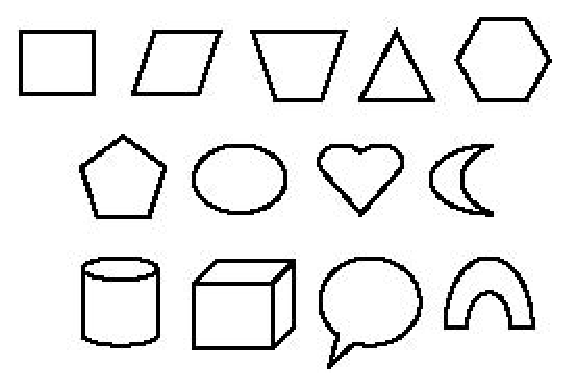
\includegraphics[scale=0.7]{images/symbolSet.eps}	}
		}
	\caption{The Symbol Set}
	\label{fig:symbolSet}
\end{figure}

\begin{figure}[]\centering
\fbox{  \parbox{8cm}{% 
		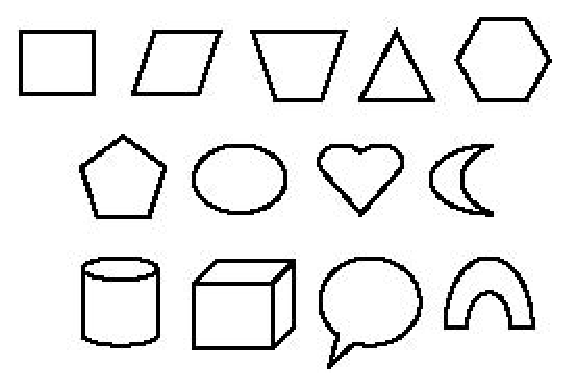
\includegraphics[scale=0.7]{images/symbolSet.eps}	}
		}
	\caption{The MultiDomain Dataset }
	\label{fig:MultisymbolSet}
\end{figure}

%\section{Evaluations techniques}
%\label{sec:EvaluationsTechniques}
%\section {Curvature estimation results}
%\label{sec:Curvatureestimationresults}


\section{Results}
\label{sec:ResultsDetails}

\subsection{PSO Algorithm}
\label{sec:PSO}
The fig. \ref{fig:dataerrorvsiteration.jpg} display the effect of the size of swarm population on the number of vertex reported while segmenting the stroke.\footnote{The fewer the vertex the better the segmentation} The graphs shows that as the number of iteration increase there is a decrease in error until the error reach a saturation and any increase in number of iteration dose not affect the error calculated. Similar behavior is noticed in fig. \ref{fig:datapopulation.jpg}.  These curves and test result in choosing the swarm parameters $c_1,c_2$ and maximum number of iteration and the swarm population. The final values are for maximum number of iteration = 150 with 15 particle for better compensation in the time domain. 

\begin{figure}
	\centering
		\includegraphics[scale=0.8]{images/dataerrorvsiteration.jpg.eps}
	\caption{Error vs. iterations }
	\label{fig:dataerrorvsiteration.jpg}
\end{figure}
\begin{figure}
	\centering
		\includegraphics[scale=0.8]{images/datapopulation.jpg.eps}
	\caption{Swarm Population }
	\label{fig:datapopulation.jpg}
\end{figure}


\subsection{Segmentation Algorithms}
\label{sec:SegmentationAlgorithms}
The result of the segmentation algorithm can be viewed in the figs. \ref{fig:results1.JPG}. These result shows the originals stroke and the segmentation that the system generated for the stroke. 
\begin{figure}
	\centering
		\includegraphics{images/results1.JPG.eps}
	\caption{Results Segmentations}
	\label{fig:results1.JPG}
\end{figure}
\begin{figure}
	\centering
		\includegraphics{images/results2.JPG.eps}
	\caption{Results Segmentaion }
	\label{fig:results2.JPG}
\end{figure}
\begin{figure}
	\centering
		\includegraphics{images/results3.JPG.eps}
	\caption{Results }
	\label{fig:results3.JPG}
\end{figure}
\begin{figure}
	\centering
		\includegraphics{images/results4.JPG.eps}
	\caption{Resluts of the segmentations}
	\label{fig:results4.JPG}
\end{figure}



The experiment we implemented was to test the effect of symbol complexity and type on the recognition rate. Figure \ref{fig:test2} shows what the accuracy of each symbol, it clearly noted that symbols that have only line segments achieve higher accuracy rate than other symbols. Figure \ref{fig:test2} also shows that algorithm 1 alone achieve better performance than algorithm 2 in the symbols that consist of lines only. The combining of both algorithm improves the recognition rate of other symbols.  \\
\begin{figure*}[]
	\centering
		\includegraphics[scale=0.5]{images/test2.eps}
	\caption{The results of second experiment}
	\label{fig:test2}
\end{figure*}
 Another experiment we performed was to test the efficiency svm classifier. We implemented the linear discriminator classifier described in \cite{gestureexample12}(see figure \ref{fig:test3}).  %The result shows that SVM is more scalable than the linear discriminator for this problem. %The test focus on the size of data needed to test each classifier and the achieved accuracy.  %For this experiment we also shows the classification time for both classifiers 
\begin{figure}[]
	\centering
		\includegraphics[scale=0.4]{images/test1.eps}
	\caption{The results of third experiment}
	\label{fig:test3}
\end{figure}
 %Details description of results got from comparing various algorithms  
 %Describe data set used for experiments ( No of data set, No. of categories, No of samples).
 %Describe other Algorithms [Alg 3 in paper \cite{earlyprocess}]used for comparing with the one described in the paper. 
 
 %In the figure \ref{fig:test1}, the accuracy means that final hit rate of all symbols used in the test set.by the  four datasets . 
We performed three experiments to test the system firstly we tested recognition accuracy of shapes in the data set with both algorithms. We also implemented the segmentation algorithm described in \cite{earlyprocess} to use as reference to our swarm algorithms.  As you see in the fig. \ref{fig:test1} shows the accuracy achieved by each algorithm. The results shows that both PSO algorithm achieve better result than other algorithms.  The swarm algorithms were tested with and without the ellipse detection module. The ellipse detection module appear to be superior to results with only the PSO algorithms.  \\  
\begin{figure}[]
	\centering
		\includegraphics[scale=0.3]{images/test1.eps}
	\caption{The results of first experiment}
	\label{fig:test1}
\end{figure}
 
%\subsection{Clustering Algorithm Results}
%\label{sec:ClusteringAlgorithmResults}

\subsection {Recognition Algorithms }
\label{sec:recognitionAlgorithms}
To test the recognition different set of features are used to select the features that will define symbols better to finally achieve better recognition rate. We tested the system using different types of features. The features explained in section \ref{sec:FeatureExtraction} was divided into different sets; statistical, structural, Rubine features and zernik moments along with composite features. The fig. \ref{fig:testFeatures} shows the result of each set of features when used with the SVM classifier. The results shows that the Rubine features although may achieve good results in single stroke symbols, have a bad performance when used with multi stroke symbols. 
\begin{figure}[]
	\centering
		\includegraphics[scale=0.3]{images/test4.eps}
	\caption{The results of Features experiment}
	\label{fig:testFeatures}
\end{figure}



We test the system using different classifier to see what the effect of the classification step on the final recognition. We also wanted to test the train and test time in both classifiers. We used SVM (RBF) classifiers and the Gaussian Linear classifier used in \cite{}. The fig. \ref{} shows the result of both classifiers with the main three segmentation algorithms. The results shows that the SVM classifier achieve better results. To measure the scalability of the system\footnote{What happens when adding a new symbols to the set of known symbols.} the classifiers are test using different number of symbols (fig. \ref{fig:sampleperCat}). Figures \ref{fig:sampleperCat} demonstrate the scalability of both classifiers by demonstrating the recognition rate in both classifiers with different number of symbols. Figures \ref{fig:sampleperCat},\ref{fig:sampleperCat} shows the time and number of symbols needed for training versus each classifier. 

\begin{figure}
	\centering
		\includegraphics{images/sampleperCat.eps}
	\caption{Samples per Category }
	\label{fig:sampleperCat}
\end{figure}

\begin{figure}
	\centering
		\includegraphics[scale=0.7]{images/test4.eps}
	\caption{Tests}
	\label{fig:test4}
\end{figure}

\section{Summary}
\label{sec:ResultSummary}

The result illustrated in this chapter shows the work done on the system and experiments performed. The results shows that the ellipse detection and PSO swarm algorithms gives better performance than other known systems. 

%\section{ BenchMark Results }
%\label{sec:BenchMarkResults}



\chapter{Discusion and Conclusion}


\section{  Conclusion}
\label{sec:ConclusionConclusion }

\section{Future Work}
\label{sec:FutureWork}



                                                % in its own file.  
%\include {Mybibliography}
\bibliography{../../neededfiles/Bibliographies/Mybibliography}     
                                                % THE APPENDIX
                                                %==============================
%\appendix                                       % Include appendix files as
  %\begin{singlespace}                           % needed or delete this block
  %\include{appendix_a}                          % of lines if no appendix.
  %\include{appendix_b}                          %
 % \include{appendix_c}                          %
%\end{singlespace}                               %


\end{document}                                  % Ends the entire document...
